\documentclass[12pt]{article}
\usepackage{amsmath, amssymb, graphicx, hyperref, float}
\usepackage[margin=1in]{geometry}
\usepackage{subcaption}
\setlength{\parindent}{0pt}

\title{AER1415: Computational Optimization\\Assignment 1\\\vspace{0.4cm}\large \textbf{University of Toronto Institute for Aerospace Studies}}
\author{Zouhair Adam Hamaimou\\Student Number: 1004981986}
\date{Due: February 14, 2025}

\begin{document}

\maketitle

\tableofcontents
\newpage

\section{Introduction}
This report presents solutions to Assignment 1 for the AER1415 course, focusing on the implementation and testing of the Particle Swarm Optimization (PSO) algorithm for constrained optimization problems. The following sections describe the PSO algorithm, parameter tuning studies using the bump test function (P3), and the application of the optimized parameters to other case studies. Additionally, solutions to the regression problem and the constraint relaxation problem are included.

\section{PSO Algorithm Implementation and Testing}

\subsection{Algorithm Description}
Particle Swarm Optimization (PSO) is a stochastic optimization algorithm inspired by the collective behavior of swarms. The algorithm maintains a population of particles, each representing a potential solution in the search space. The particles adjust their positions based on their own experiences and the experiences of their neighbors.
\\
For the following general constrained optimization problem:
\begin{equation*}
    \begin{aligned}
        \text{Minimize:} \quad & f(\mathbf{x}) \\
        \text{Subject to:} \quad & g_i(\mathbf{x})  \leq 0, \quad i = 1, \dots, m, \\
        & h_j(\mathbf{x})  = 0, \quad j = 1, \dots, q, \\
        & \mathbf{x}  \in \mathcal{X} \subset \mathbb{R}^n,
    \end{aligned}
\end{equation*}

The main steps of the PSO algorithm are as follows:
\begin{enumerate}
    \item Initialize a swarm of particles with random positions $\mathbf{x}_{i}(t=0)$ and velocities $\mathbf{v}_{i}(t=0)$ within the defined bounds.
    \item Evaluate the objective function value $f(\mathbf{x}_i)$ for each particle.
    \item Update each particle's personal best position $\mathbf{p}_{i,\text{best}}$ and the global best position $\mathbf{g}_{\text{best}}$.
    \item Update the velocity and position of each particle using:
    \begin{align*}
        \mathbf{v}_{i}(t+1) &= w \mathbf{v}_{i}(t) + c_1 \mathbf{r}_1 \odot (\mathbf{p}_{i,\text{best}} - \mathbf{x}_{i}(t)) + c_2 \mathbf{r}_2 \odot (\mathbf{g}_{\text{best}} - \mathbf{x}_{i}(t)), \\
        \mathbf{x}_{i}(t+1) &= \mathbf{x}_{i}(t) + \mathbf{v}_{i}(t+1),
    \end{align*}
    where $w$ is the inertia weight, $c_1$ and $c_2$ are acceleration coefficients, and $\mathbf{r}_1$ and $\mathbf{r}_2$ are random vectors whose elements are uniformly distributed in the interval $[0,1]$.
    \item Repeat steps 2--4 until the maximum number of iterations is reached or the improvement in the objective value is less than the specified tolerance for a defined number of consecutive iterations.
\end{enumerate}

To handle constraints, the quadratic penalty function approach is employed:
\begin{equation*}
    \phi(\mathbf{x}) = \sum_{i=1}^{m} \max(0, g_i(\mathbf{x}))^2 + \sum_{i=1}^{q} h_i(\mathbf{x})^2,
\end{equation*}
The penalty is added to the objective function value using a static or adaptive penalty coefficient to discourage infeasible solutions. The static penalty method applies a fixed penalty parameter $\lambda$ throughout the optimization process. The penalized objective function is given by:
\begin{equation*}
    F(\mathbf{x}) = f(\mathbf{x}) + \rho \phi(\mathbf{x}),
\end{equation*}
where a large $\rho$ discourages constraint violations but may hinder exploration. This method is simple but may require careful tuning of $\rho$ to balance feasibility and convergence. The adaptive penalty method dynamically adjusts the penalty coefficient based on the iteration count or constraint violations. A commonly used adaptive penalty function is:
\begin{equation*}
    F(\mathbf{x}, t) = f(\mathbf{x}) + (C (t + 1))^{\alpha} \phi(\mathbf{x}),
\end{equation*}
where $C$ is a scaling factor, $t$ is the iteration number, and $\alpha$ controls the rate of penalty increase. This method allows the optimizer to explore the search space more freely in early iterations and gradually enforce feasibility as the optimization progresses.

\subsection{Parameter Tuning Studies}
The bump test function (\textbf{P3}) was used to tune the parameters of the Particle Swarm Optimization (PSO) algorithm. The function is defined as:
\begin{align*}
    \text{Minimize:} & \quad -\left|\sum_{i=1}^{n} \cos^4(x_i) - 2 \prod_{i=1}^{n} \cos^2(x_i) \right| \Big/ \sqrt{\sum_{i=1}^{n} i x_i^2}, \\
    \text{Subject to:} & \quad \prod_{i=1}^{n} x_i > 0.75, \quad \sum_{i=1}^{n} x_i < 15n/2, \quad 0 \leq x_i \leq 10.
\end{align*}

The goal of this section is to optimize the PSO hyperparameters for this function. The parameters tuned include:
\begin{itemize}
    \item Number of particles ($n_p$)
    \item Inertia weight ($w$)
    \item Cognitive coefficient ($c_1$)
    \item Social coefficient ($c_2$)
    \item Static penalty parameter ($\rho$) for the static penalty method
    \item Adaptive penalty parameters ($C$ and $\alpha$) for the adaptive penalty method
\end{itemize}

\subsubsection*{Hyperparameter Optimization Procedure}
The performance of PSO with the specified hyperparameters was evaluated over 10 independent runs. The search space for the hyperparameters was defined as follows:
\begin{itemize}
    \item Penalty method: \{Static, Adaptive\}
    \item $n_p$: Integer in [10, 60]
    \item $w$: Real in [0.4, 1.4]
    \item $c_1$: Real in [1.5, 2.0]
    \item $c_2$: Real in [2.0, 2.5]
    \item $\rho$: Integer in [$10^2$, $10^4$] (Static penalty only)
    \item $C$: Real in [0.5, 1.0] (Adaptive penalty only)
    \item $\alpha$: Real in [1.0, 2.0] (Adaptive penalty only)
\end{itemize}

The \texttt{gp\_minimize} function from the \texttt{scikit-optimize} library was used to perform Bayesian optimization with Gaussian process regression. The hyperparameter search involved:
\begin{itemize}
    \item 200 total evaluations (\texttt{n\_calls=200})
    \item 20 random initial configurations (\texttt{n\_random\_starts=20})
    \item Parallelized evaluations (\texttt{n\_jobs=-1})
\end{itemize}

The best hyperparameters obtained for each penalty method are summarized in the following tables:

\begin{table}[h!]
\centering
\caption{Top 3 Hyperparameter Configurations for STATIC Penalty Method}
\begin{tabular}{|c|c|c|c|c|c|c|}
\hline
$n_p$ & $w$ & $c_1$ & $c_2$ & $\rho$ & Best solution & Function value \\
\hline
59 & 0.406 & 1.527 & 2.135 & 7535 & [1.60088, 0.4685] & -0.36498 \\
59 & 0.499 & 1.527 & 2.014 & 2855 & [1.60076, 0.46854] & -0.36497 \\
13 & 0.412 & 1.985 & 2.071 & 9414 & [1.60133, 0.46861] & -0.36477 \\
\hline
\end{tabular}
\end{table}

\begin{table}[h!]
\centering
\caption{Top 3 Hyperparameter Configurations for ADAPTIVE Penalty Method}
\begin{tabular}{|c|c|c|c|c|c|c|c|}
\hline
$n_p$ & $w$ & $c_1$ & $c_2$ & $C$ & $\alpha$ & Best solution & Function value \\
\hline
42 & 0.625 & 1.968 & 2.001 & 0.50 & 1.94 & [1.59319, 0.48156] & -0.35564 \\
60 & 0.726 & 1.988 & 2.003 & 0.57 & 1.98 & [1.68511, 0.46405] & -0.34221 \\
59 & 1.355 & 1.974 & 2.481 & 0.98 & 1.44 & [1.50011, 0.53947] & -0.31763 \\
\hline
\end{tabular}
\end{table}

\subsubsection*{Convergence Trends}
The convergence plots for the best configurations of each penalty method are shown below. These plots illustrate the mean convergence trend over 10 independent runs, with a confidence interval of $\pm$3 standard deviations.

\begin{figure}[b!]
    \centering
    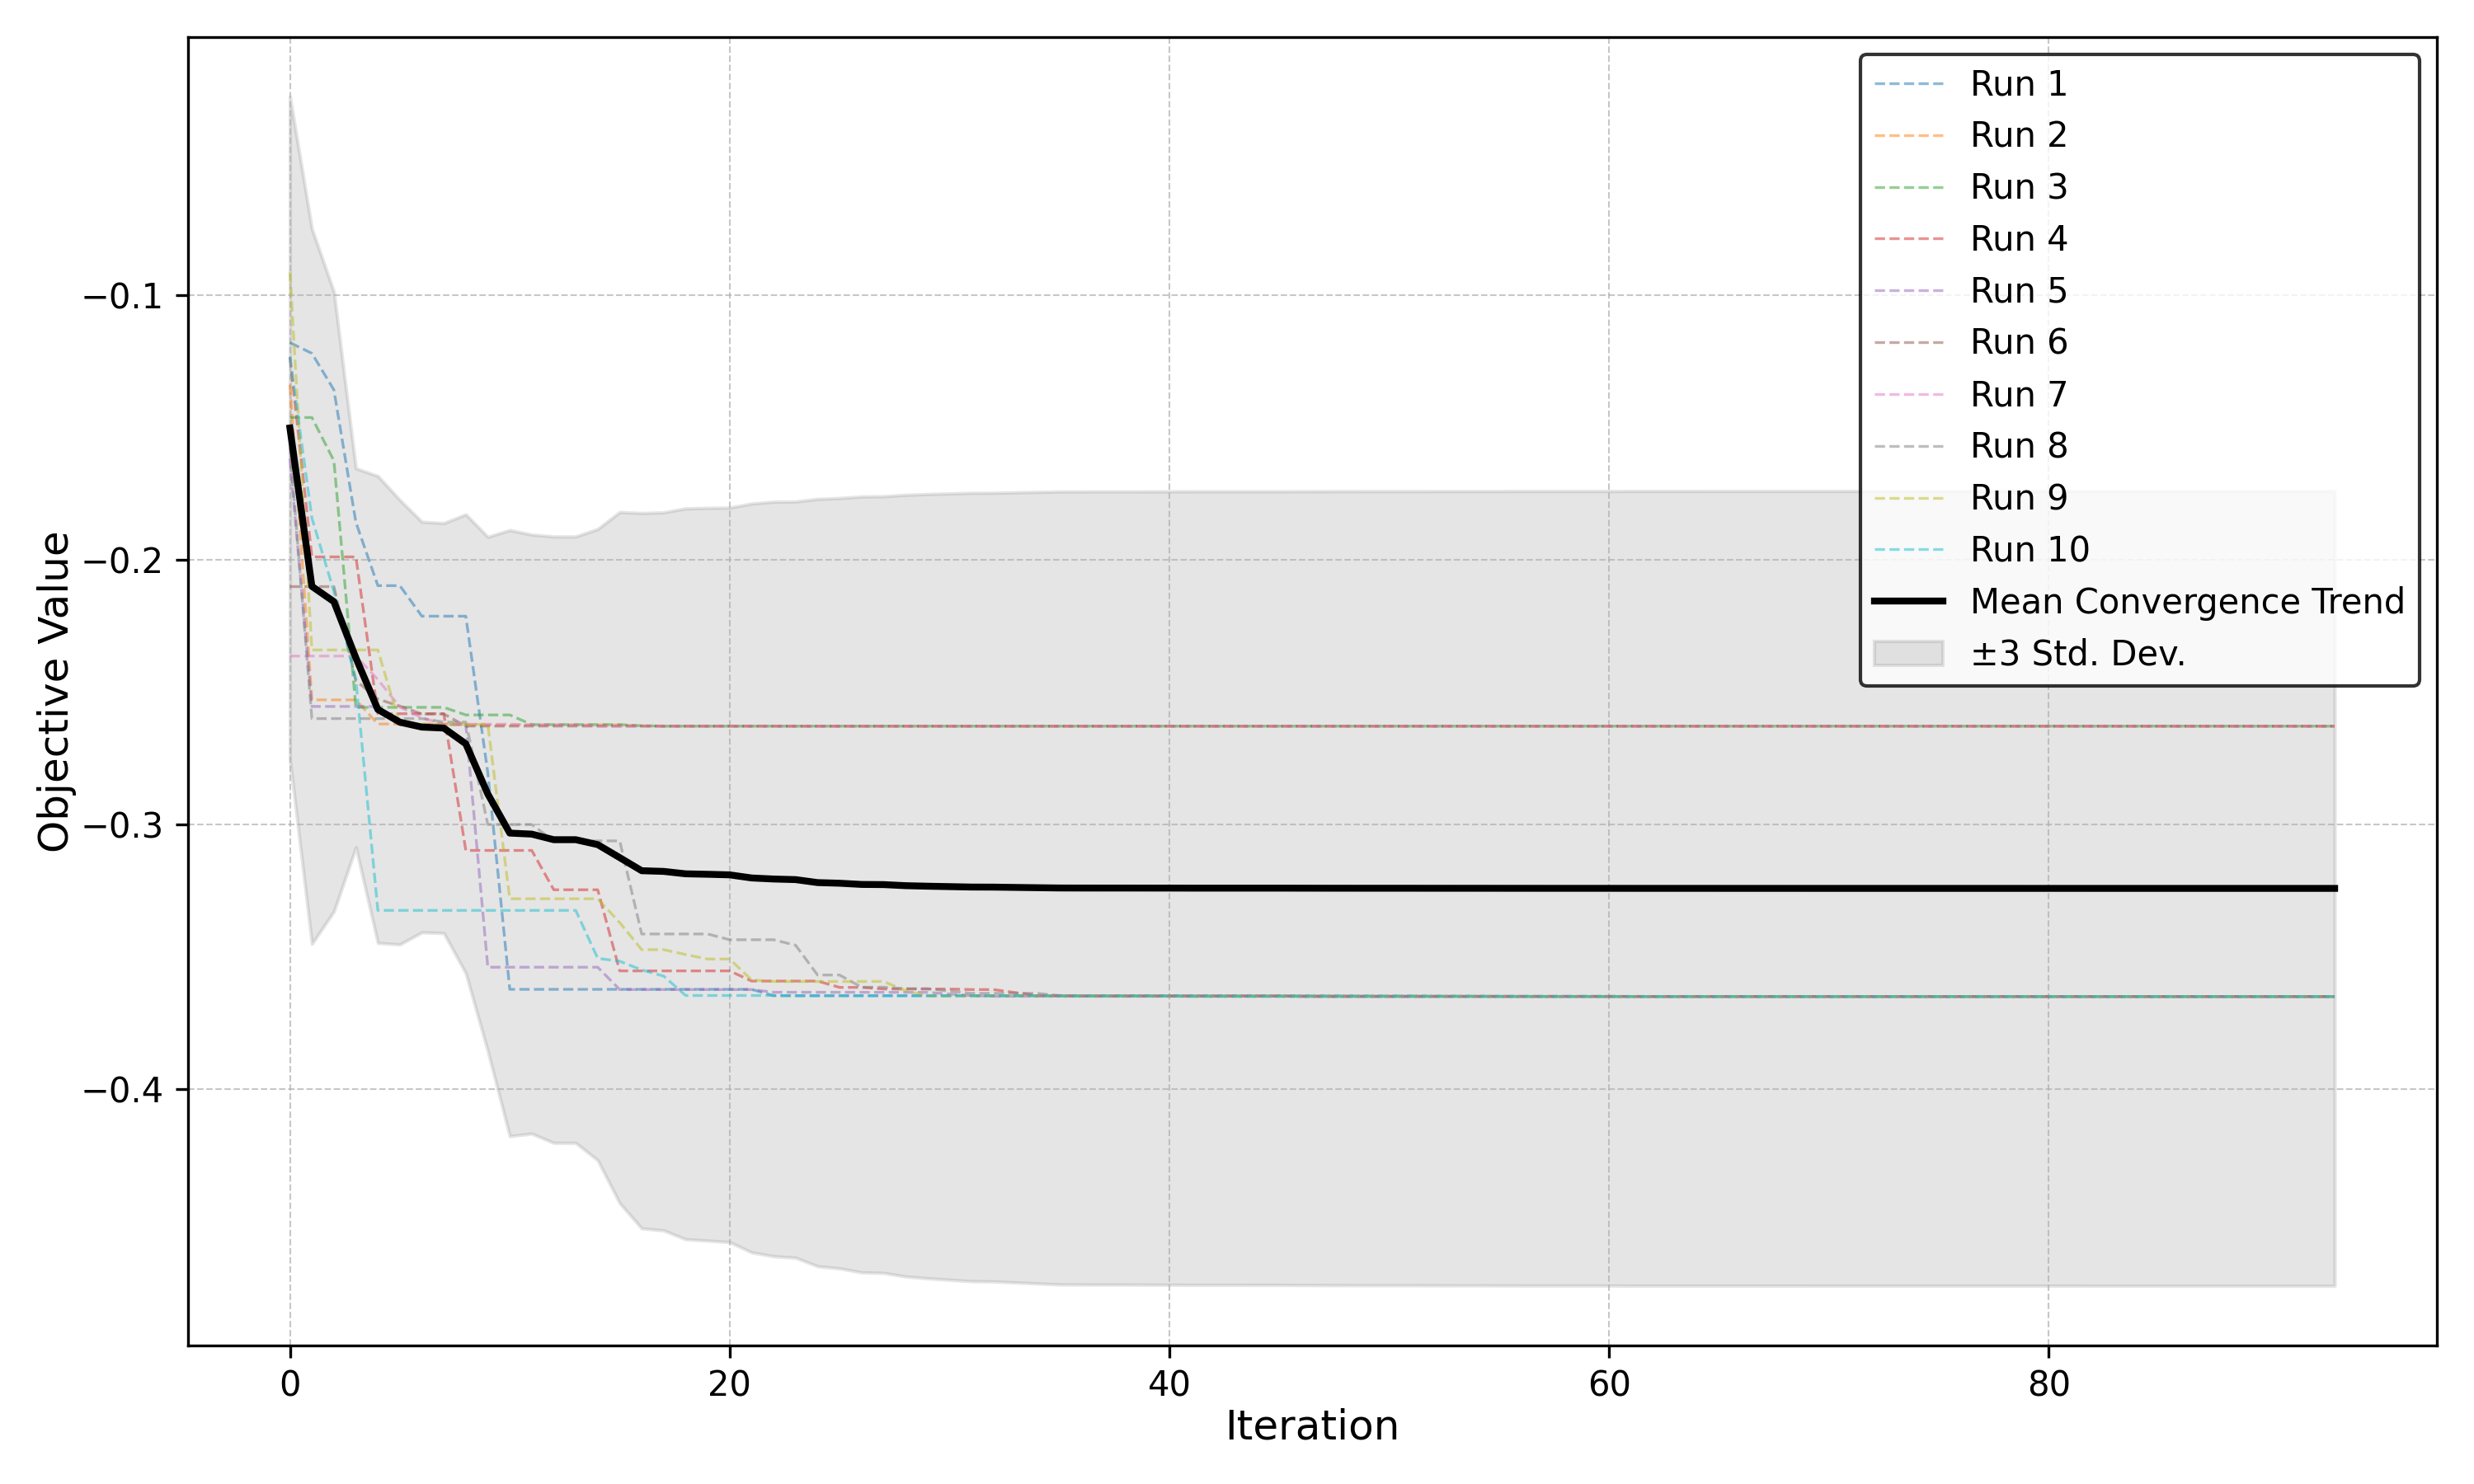
\includegraphics[width=0.8\textwidth]{../best_plots/P3_2D_STATIC_convergence_n59_w0.4063759899463055_c11.527326152164539_c22.1348929944802615_STATIC_rho7535.190137383015.png}
    \caption{Convergence plot for the best STATIC penalty method configuration}
    \label{fig:static_pso}
\end{figure}

\begin{figure}[b!]
    \centering
    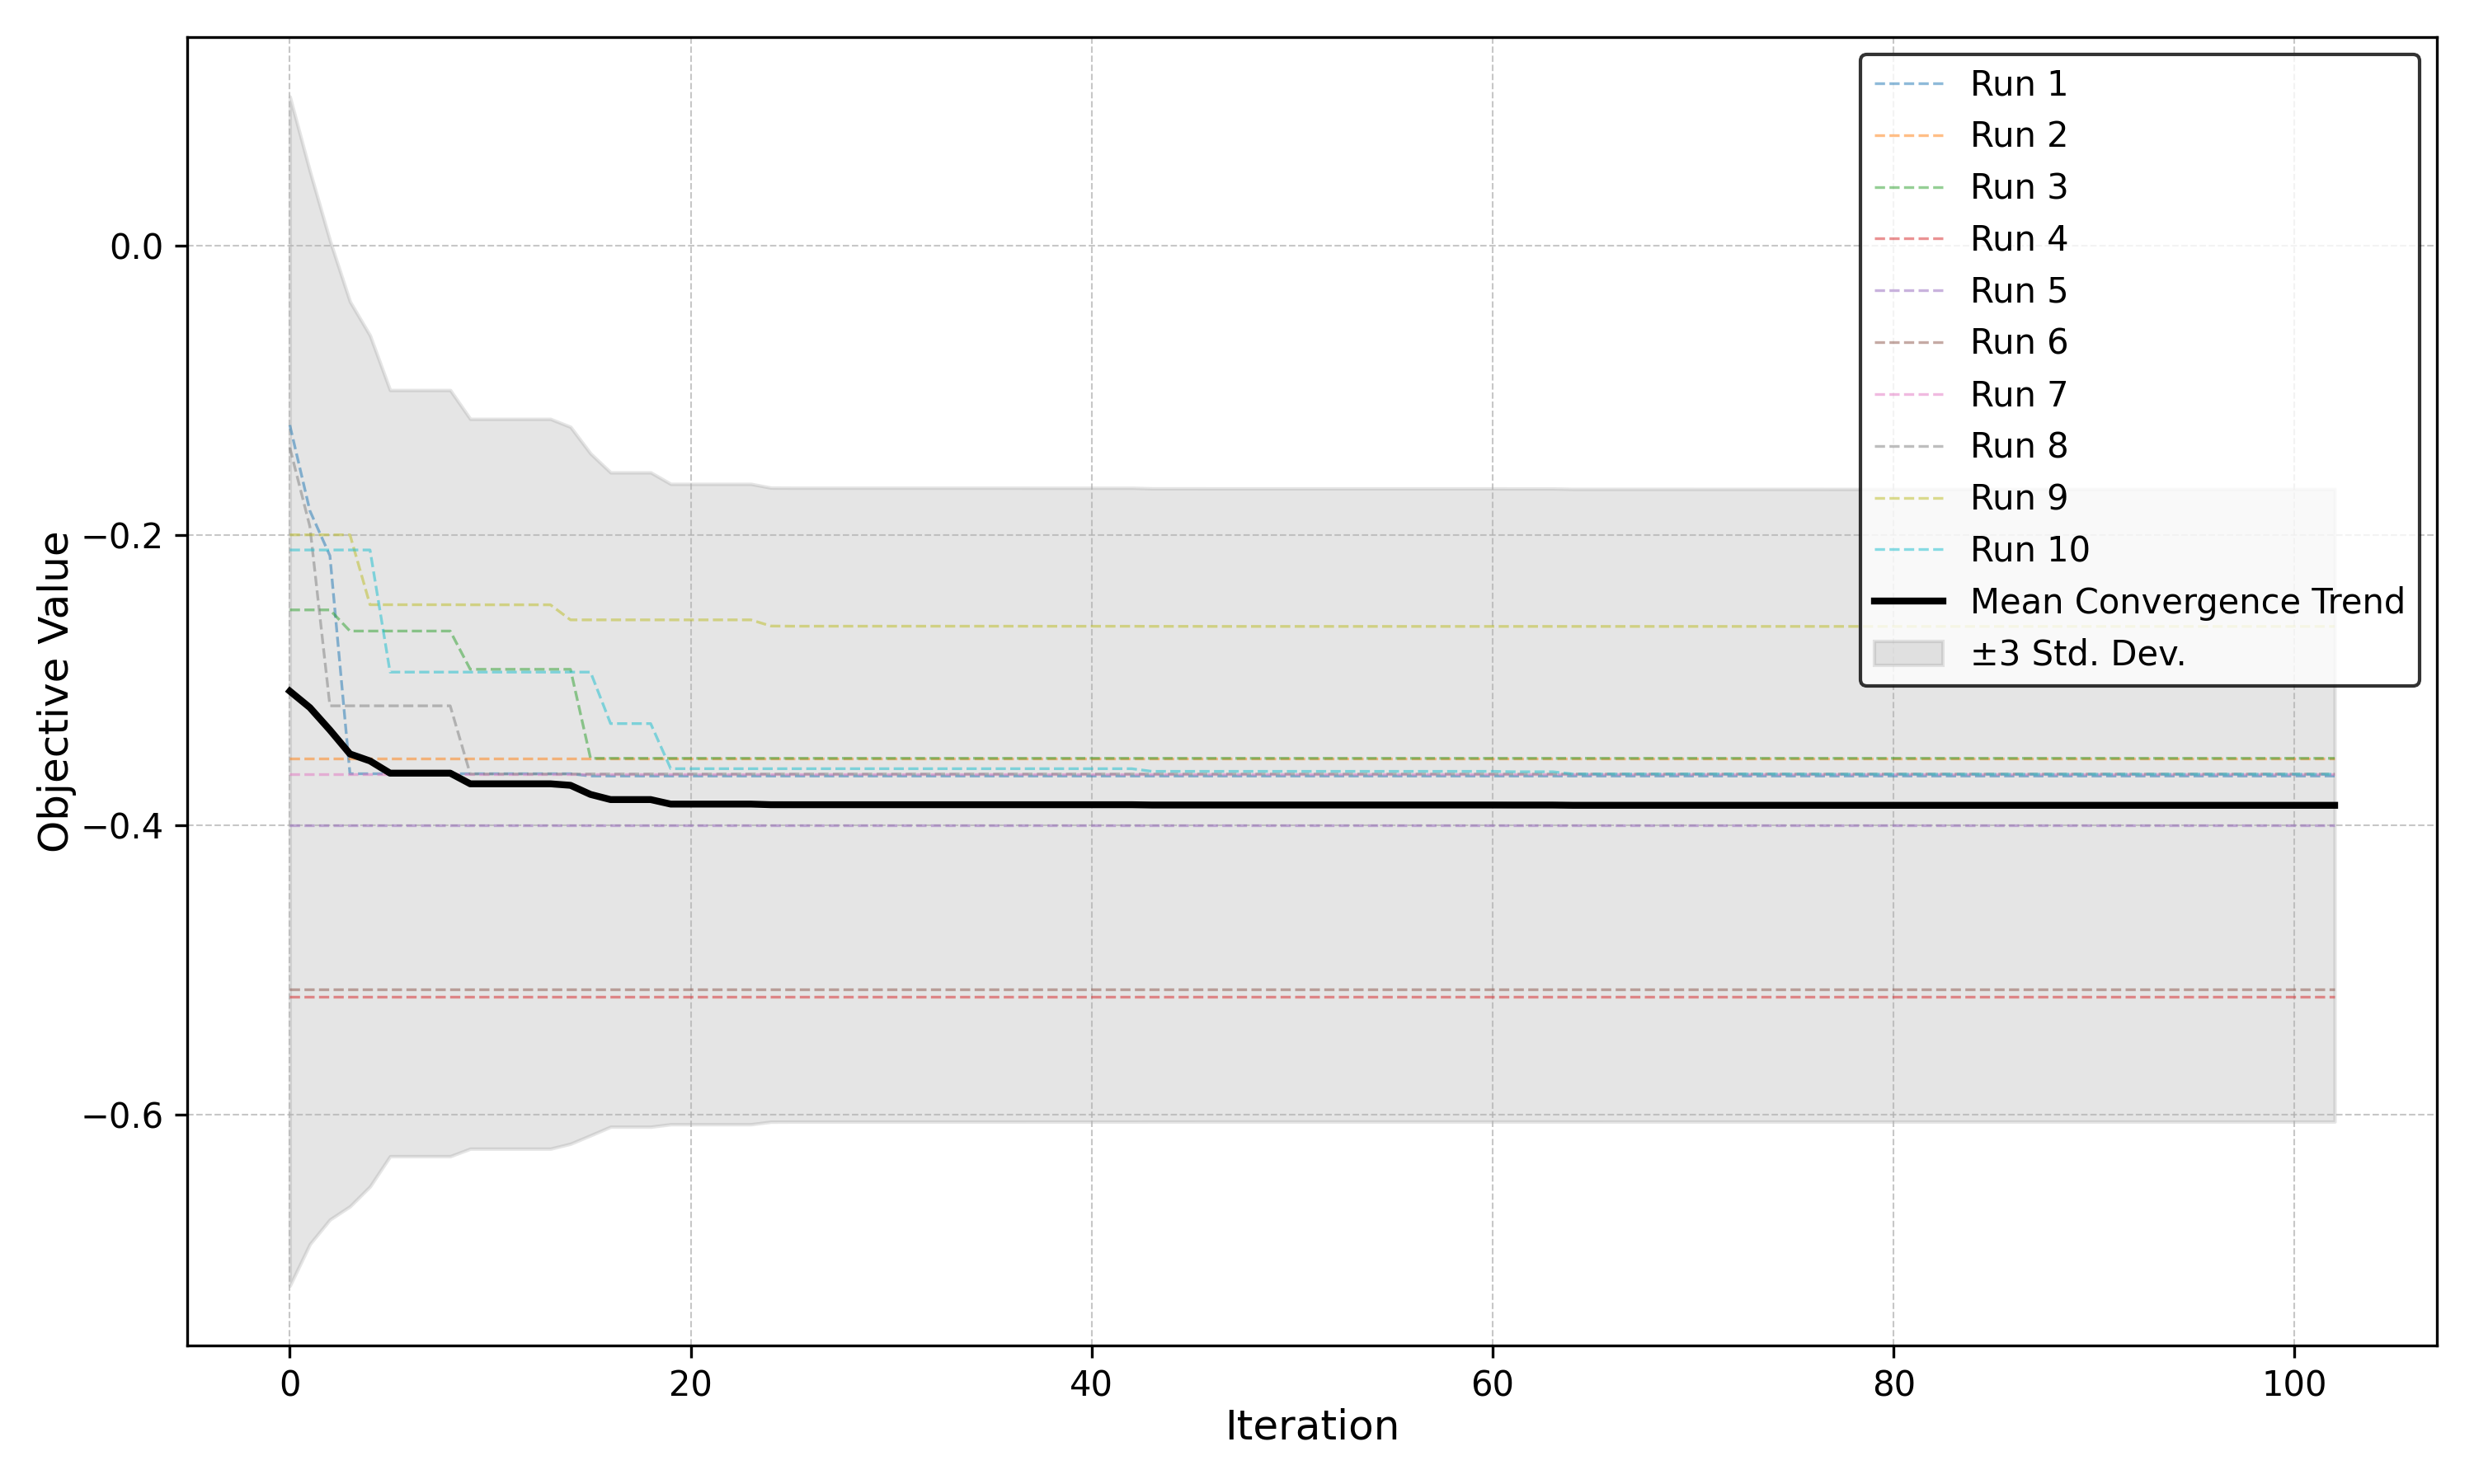
\includegraphics[width=0.8\textwidth]{../best_plots/P3_2D_ADAPTIVE_convergence_n42_w0.6248024703859039_c11.9679646120707424_c22.0006087252924303_ADAPTIVE_C0.5040335872985765_alpha1.938183640589161.png}
    \caption{Convergence plot for the best ADAPTIVE penalty method configuration}
    \label{fig:adaptive_pso}
\end{figure}

\subsubsection*{Summary}
From the results, the static penalty method achieved slightly better convergence performance for the bump test function (\textbf{P3}), with a best function value of $-0.36498$. However, the adaptive penalty method showed comparable performance with a best function value of $-0.35564$. The following tuned hyperparameters will be used in subsequent case studies to assess performance on other constrained optimization problems:
\begin{itemize}
    \item Penalty method: Static
    \item $n_p$: 59
    \item $w$: 0.406
    \item $c_1$: 1.527
    \item $c_2$: 2.135
    \item $\rho$: 7535
\end{itemize}
\subsection{Results for Case Studies}
The tuned PSO parameters were applied to additional case studies from the "Case Studies" document. Results include the best solution found, the corresponding objective function value, and the feasibility of the solution. Detailed convergence plots and solution statistics are included for each case study.

\subsubsection{P1: Minimization of the Rosenbrock Function}
The Rosenbrock test function was minimized for both 2-dimensional and 5-dimensional cases. The problem is defined as:
\begin{align*}
    \text{Minimize:} & \quad f(\mathbf{x}) = \sum_{i=1}^{n-1} \left[100(x_{i+1} - x_i^2)^2 + (1 - x_i)^2\right], \\
    \text{Subject to:} & \quad -5 \leq x_i \leq 5, \quad i = 1, 2, \dots, n.
\end{align*}

\paragraph{2-Dimensional Case}
The PSO algorithm successfully minimized the Rosenbrock function in 2 dimensions, achieving the following results:
\begin{itemize}
    \item \textbf{Best solution:} $[0.9999, 0.9997]$
    \item \textbf{Best objective value:} $2.67 \times 10^{-8}$
\end{itemize}

\begin{figure}[h!]
    \centering
    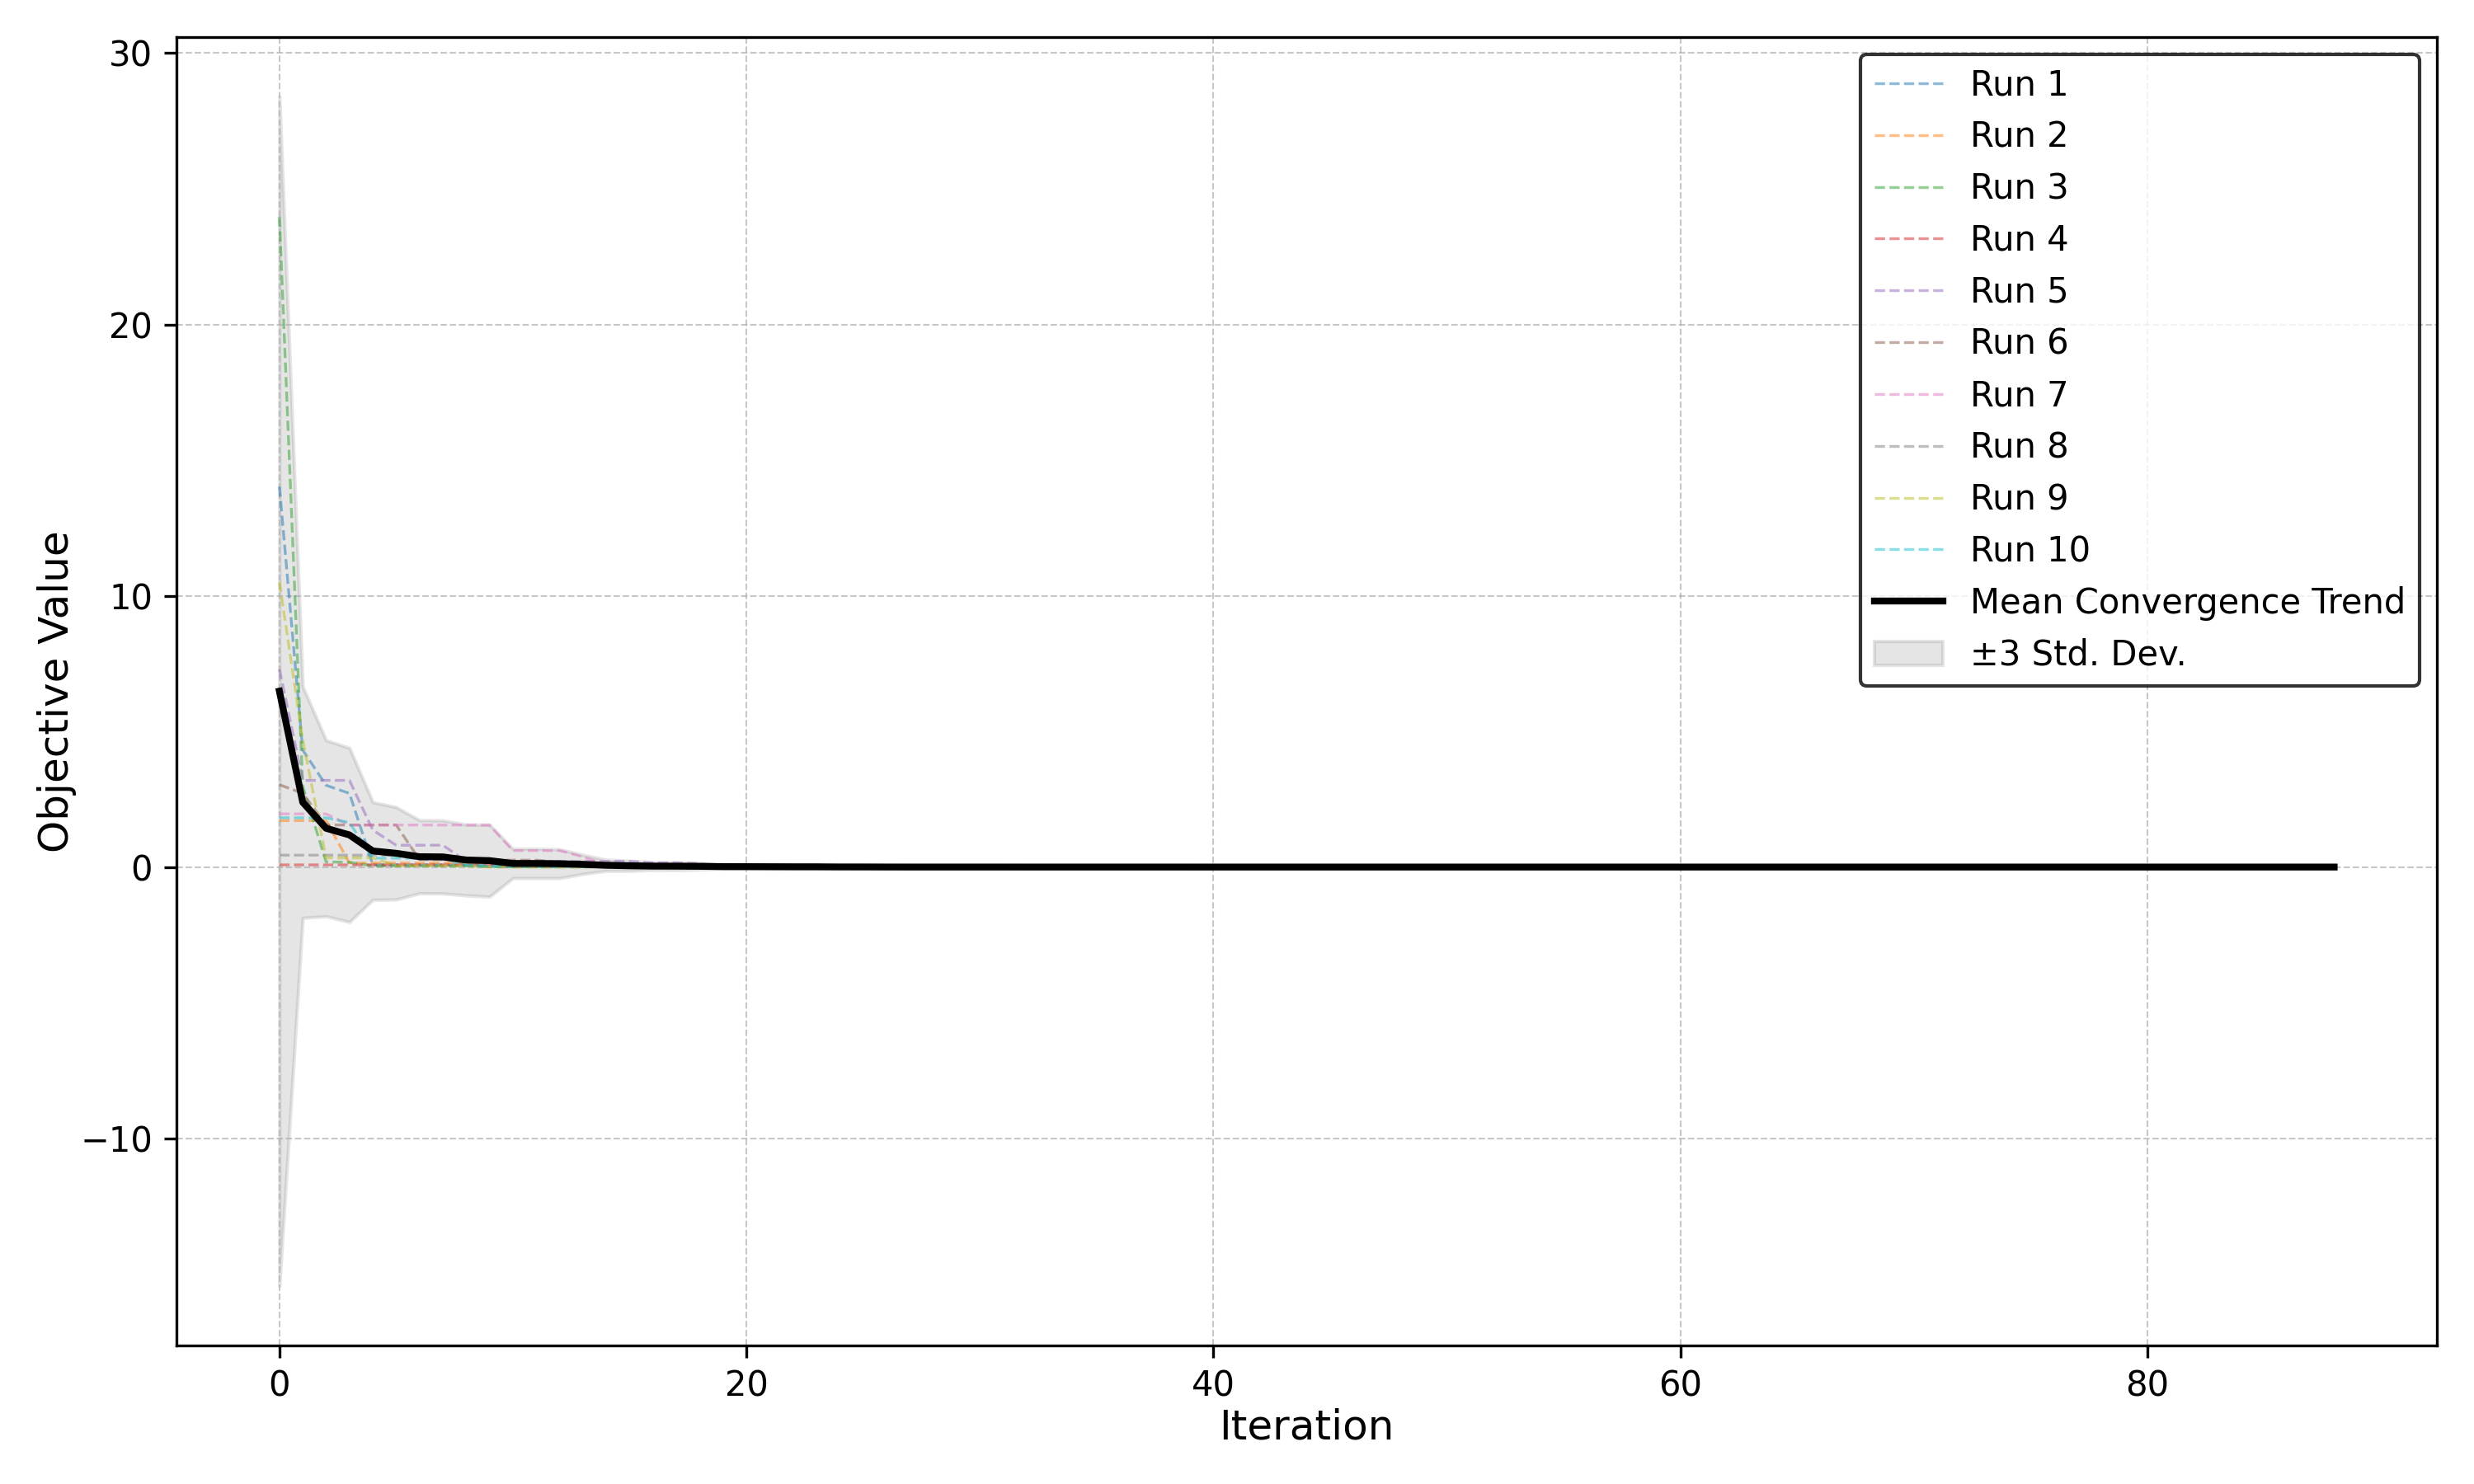
\includegraphics[width=0.8\textwidth]{../best_plots/P1_2D_convergence_n59_w0.406_c11.527_c22.135_STATIC_rho7535.png}
    \caption{Convergence plot for P1 2D (2-dimensional Rosenbrock function)}
    \label{fig:p1_2d_convergence}
\end{figure}

\paragraph{5-Dimensional Case}
For the 5-dimensional case, the PSO algorithm required an increased number of iterations (maximum iterations set to 1000) to achieve convergence. The results are as follows:
\begin{itemize}
    \item \textbf{Best solution:} $[0.9952, 0.9907, 0.9819, 0.9640, 0.9294]$
    \item \textbf{Best objective value:} $0.00176$
\end{itemize}

\begin{figure}[h!]
    \centering
    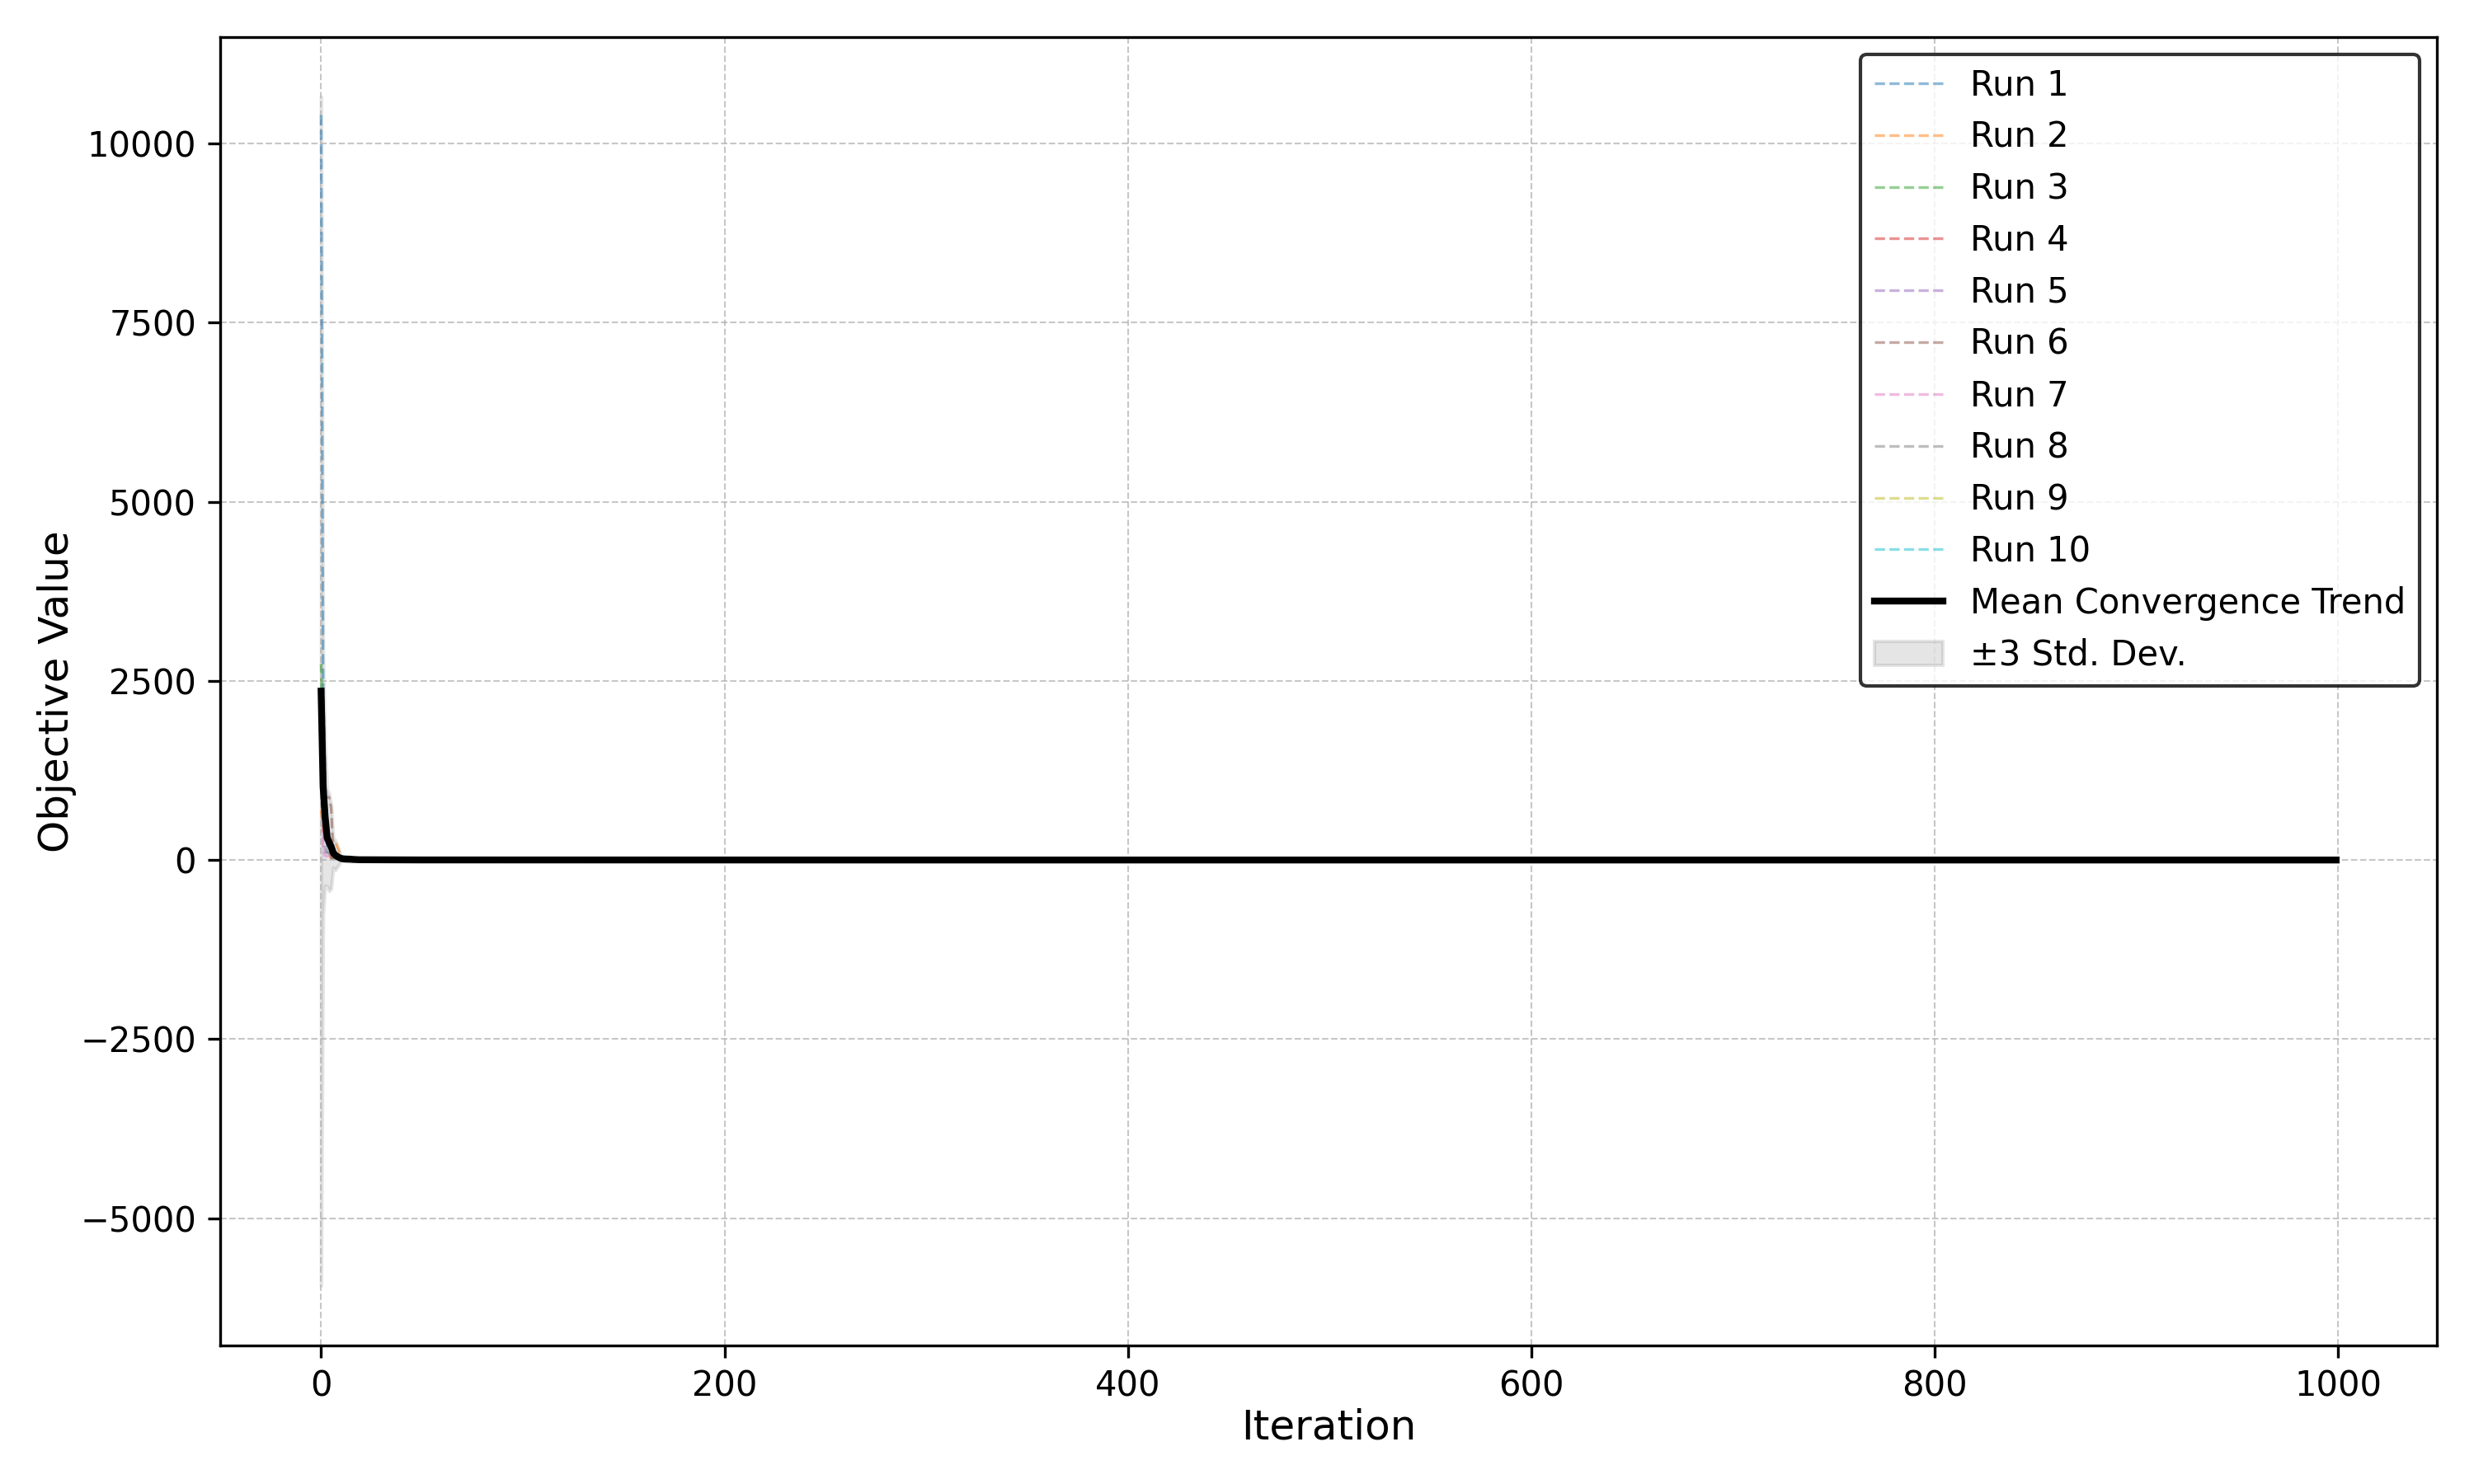
\includegraphics[width=0.8\textwidth]{../best_plots/P1_5D_convergence_n59_w0.406_c11.527_c22.135_STATIC_rho7535.png}
    \caption{Convergence plot for P1 5D (5-dimensional Rosenbrock function)}
    \label{fig:p1_5d_convergence}
\end{figure}

\paragraph{Commentary on Results}
The results demonstrate that the tuned PSO parameters perform well in optimizing the Rosenbrock function. For the 2-dimensional case, the objective value achieved was close to zero, indicating near-perfect convergence to the global minimum. In the 5-dimensional case, the algorithm converged to a slightly higher objective value, which is expected due to the increased dimensionality and complexity of the problem. The convergence trends in both cases show smooth progress toward the optimal solution, with no major oscillations or divergence.

\subsubsection{P2: Constrained Optimization Problem (Algebraic in 2 Variables)}
The constrained optimization problem P2 was solved using the tuned PSO parameters. The problem is defined as:
\begin{align*}
    \text{Minimize:} & \quad f(\mathbf{x}) = x_1^2 + 0.5x_1 + 3x_1x_2 + 5x_2^2, \\
    \text{Subject to:} & \quad 3x_1 + 2x_2 + 2 \leq 0, \\
                      & \quad 15x_1 - 3x_2 - 1 \leq 0, \\
                      & \quad -1 \leq x_1 \leq 1, \\
                      & \quad -1 \leq x_2 \leq 1.
\end{align*}

The PSO algorithm successfully converged to a solution within the specified tolerance. The results are as follows:
\begin{itemize}
    \item \textbf{Best solution:} $[-0.8059, 0.2089]$
    \item \textbf{Best objective value:} $-0.04032$
    \item \textbf{Constraints: } $3x_1 + 2x_2 + 2 \approx -7.87 \times 10^{-5}$ and  $5x_1 - 3x_2 - 1 \approx -13.73$
\end{itemize}

The convergence plot for this problem is shown below:

\begin{figure}[h!]
    \centering
    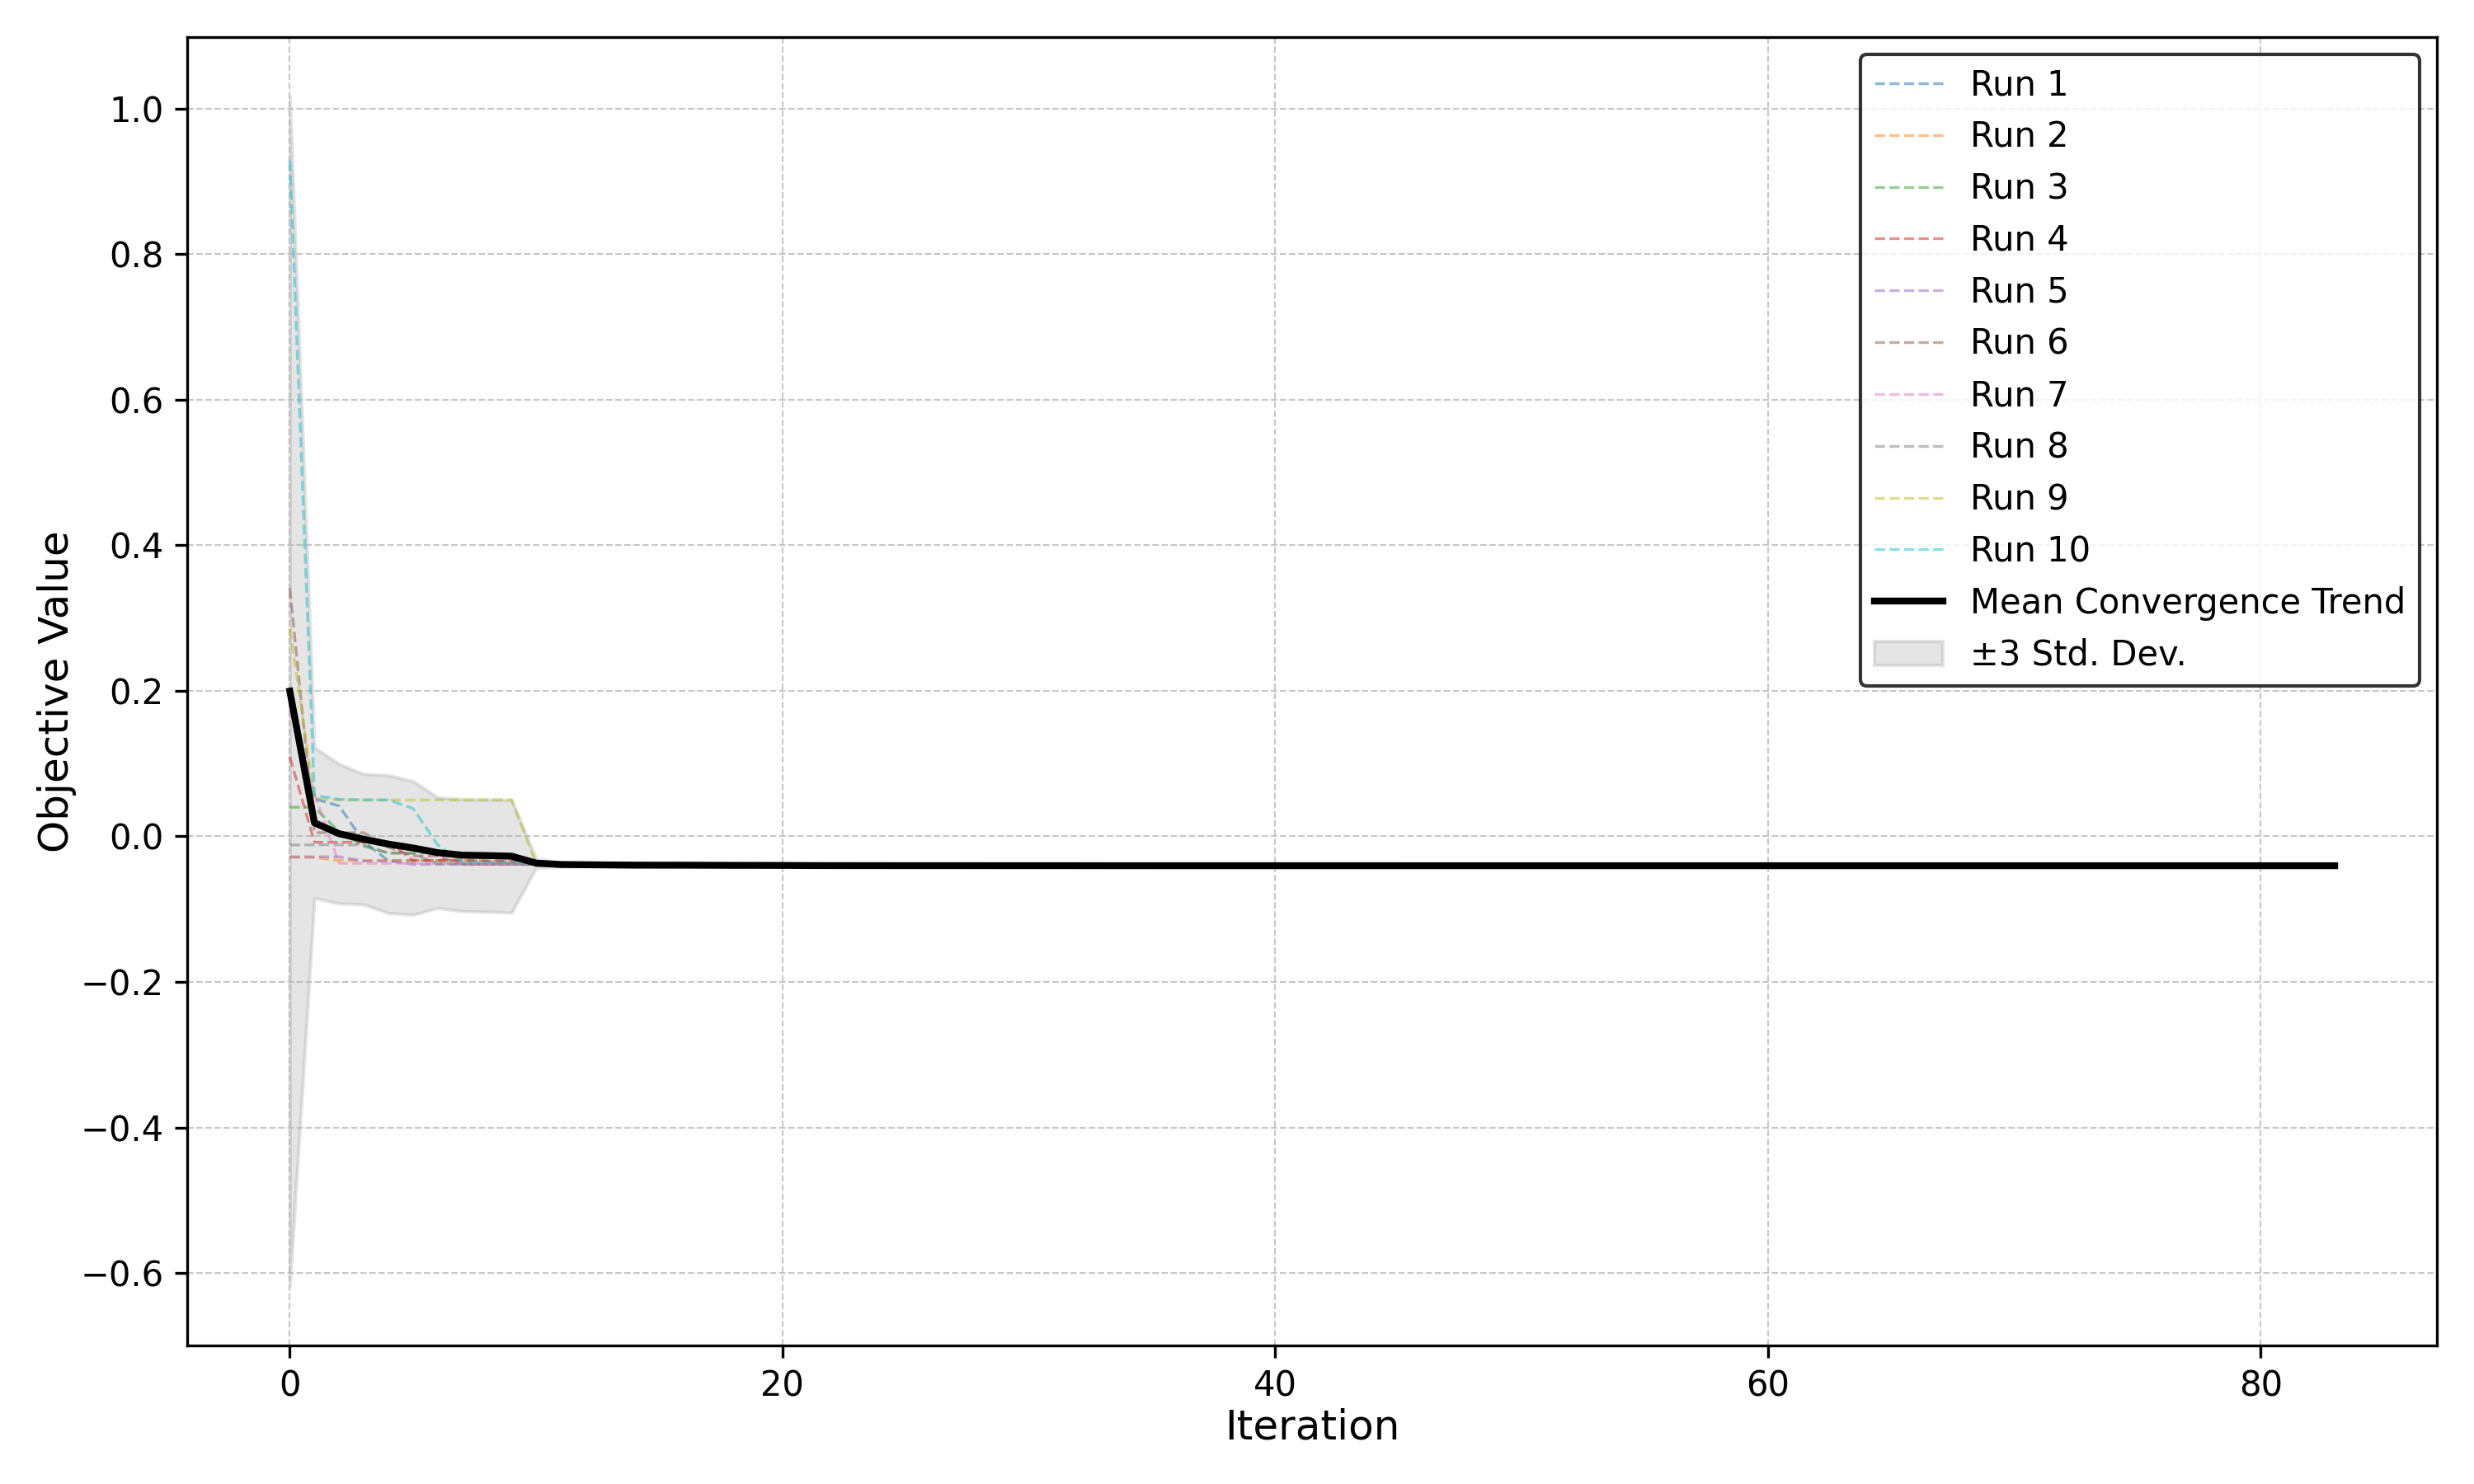
\includegraphics[width=0.8\textwidth]{../best_plots/P2_2D_convergence_n59_w0.406_c11.527_c22.135_STATIC_rho7535.png}
    \caption{Convergence plot for P2 (Constrained optimization problem in 2 variables)}
    \label{fig:p2_convergence}
\end{figure}

\paragraph{Commentary on Results}
The PSO algorithm effectively handled the constraints of the problem using the static penalty method. The best solution found is feasible, satisfying all constraints. The convergence plot demonstrates steady improvement toward the optimal solution, achieving convergence within the tolerance threshold. The negative objective value indicates the minimization of the function was successful under the given constraints.

\subsection{Results for P3: Constrained Bump Test Function}
The analysis for the 2-dimensional case of the bump test function (\textbf{P3}) was provided in the parameter tuning studies section. This section presents the results for the 10-dimensional case (\(n = 10\)) of \textbf{P3}.

The optimization was performed with a maximum of 300 iterations and a patience of 25 consecutive iterations to reach the tolerance threshold. The results for the 10-dimensional case are as follows:
\begin{itemize}
    \item \textbf{Best solution:} [3.1217, 3.0709, 3.0136, 2.9659, 1.4663, 0.3645, 0.3612, 0.3601, 0.3621, 0.3477]
    \item \textbf{Best objective value:} $-0.7473$
    \item \textbf{Constraint 1 value:} $0.75 - \prod_{i=1}^{n} x_i = -0.0001$
    \item \textbf{Constraint 2 value:} $\sum_{i=1}^{n} x_i - 15n/2 = -59.5660$ 
\end{itemize}

The convergence trend for this optimization is shown in Figure~\ref{fig:p3_10d_convergence}. The plot demonstrates the mean convergence trend over 10 independent runs, with a confidence interval of $\pm$3 standard deviations.

\begin{figure}[h]
    \centering
    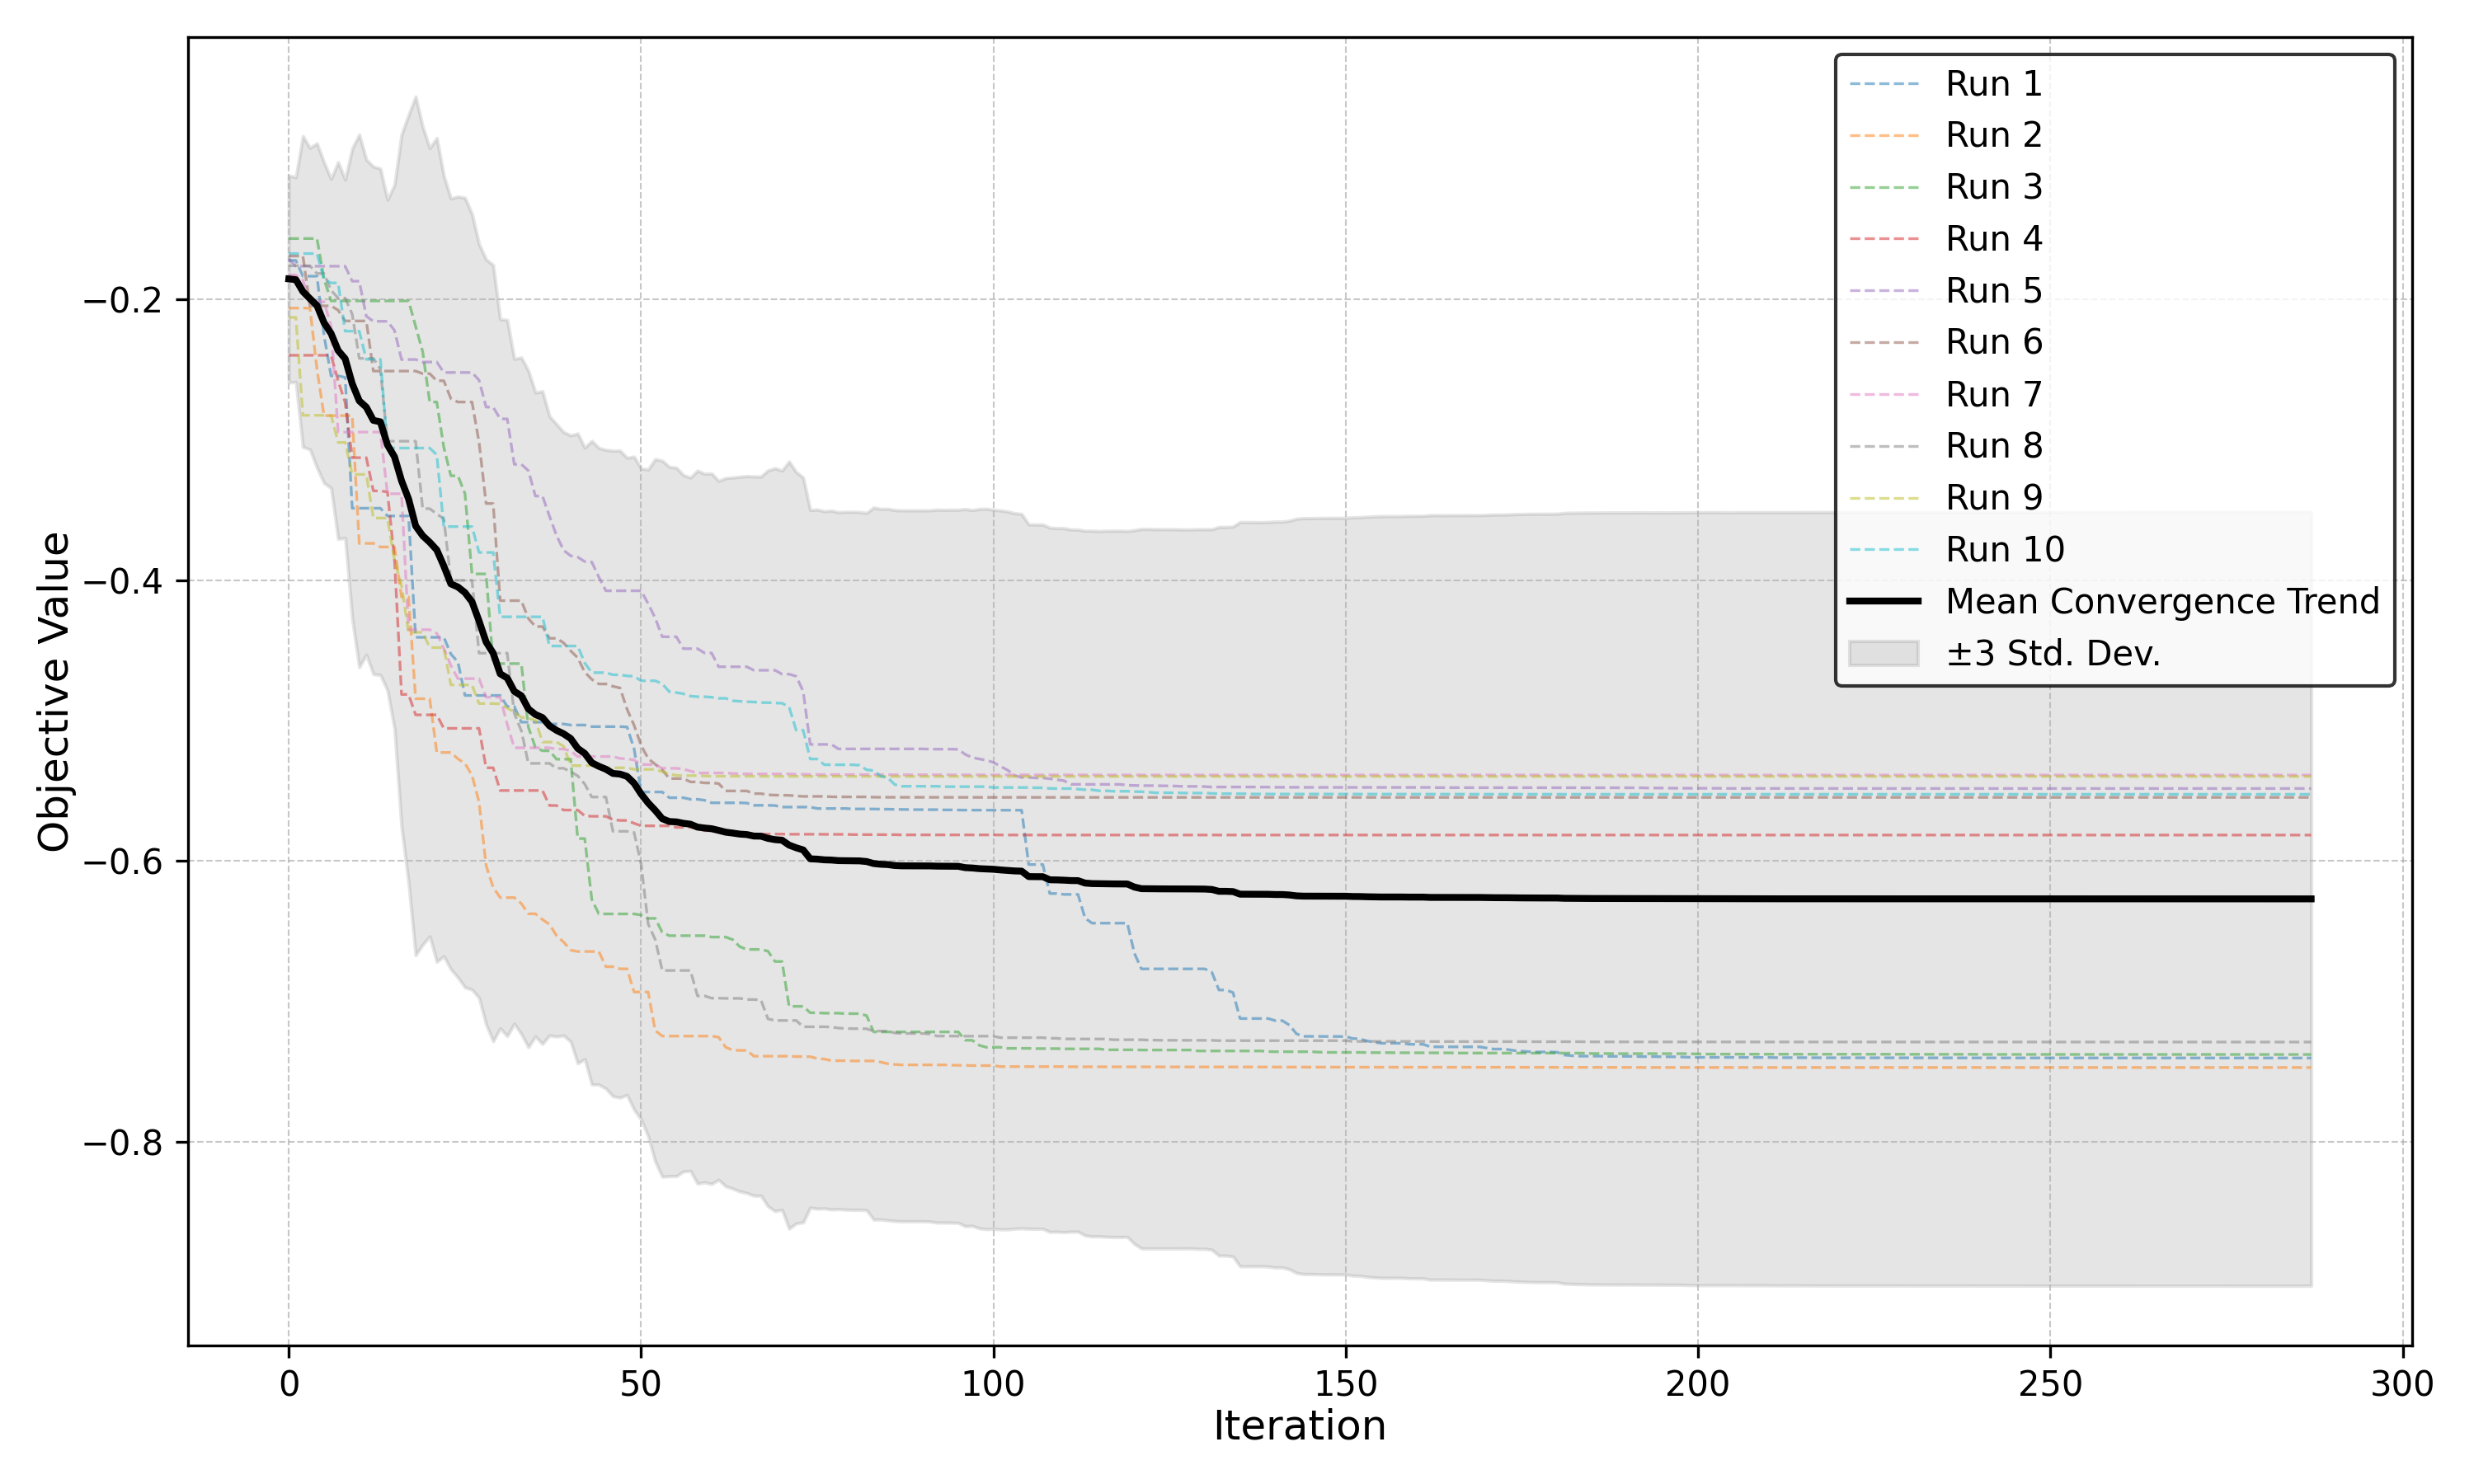
\includegraphics[width=0.8\textwidth]{../best_plots/P3_10D_convergence_n59_w0.406_c11.527_c22.135_STATIC_rho7535.png}
    \caption{Convergence plot for \textbf{P3} with \(n = 10\) using the tuned PSO parameters.}
    \label{fig:p3_10d_convergence}
\end{figure}

\subsection{P4: Brachistochrone Problem}
The Brachistochrone problem is a classic test case in optimization and was originally solved analytically by Johann Bernoulli. The objective is to determine the path between two points such that the travel time of a particle under the influence of gravity is minimized. For this study, the starting and ending points are specified as $(x_1, y_1) = (0, 1)$ and $(x_n, y_n) = (1, 0)$, respectively, and the coefficient of kinetic friction is set to $\mu_k = 0$.

\subsubsection{Problem Formulation}
To discretize the problem, the path is divided into $n$ line segments, and the coordinates of the intermediate points are parametrized. The objective function for the total travel time is expressed as:
\begin{align*}
    T &= \sum_{i=1}^{n-1} \Delta t_i, \\
    \Delta t_i &= \frac{\sqrt{\Delta x_i^2 + \Delta y_i^2}}{\sqrt{h - y_{i+1} - \mu_k x_{i+1}} + \sqrt{h - y_i - \mu_k x_i}},
\end{align*}
where:
\begin{itemize}
    \item $\Delta x_i = \frac{x_n - x_1}{n-1} = \frac{1}{n-1}$ is the horizontal distance between consecutive points,
    \item $\Delta y_i = y_{i+1} - y_i$ is the vertical distance between consecutive points,
    \item $h = 1$ is the height of the starting point.
\end{itemize}

The goal is to minimize $T$ by varying the $y$-coordinates of the intermediate points, $y_i$ $(i = 2, \ldots, n-1)$, while keeping the first and last points fixed. This results in $n-2$ design variables, which we respresent compactly with the vector $\mathbf{y} = \begin{bmatrix}y_2 & \ldots & y_{n-1}\end{bmatrix}^T$.

The optimization problem can be written as:
\begin{align*}
    \text{Find:} & \quad \arg \min_{\mathbf{y} \in \mathbb{R}^{n-2}} T(\mathbf{y}) = \arg \min_{\mathbf{y} \in \mathbb{R}^{n-2}} \sum_{i=1}^{n-1} \frac{\sqrt{\Delta x_i^2 + \Delta y_i^2}}{\sqrt{h - y_{i+1}} + \sqrt{h - y_i}}, \\
    \text{Subject to:} & \quad 0 \leq y_i \leq 1, \quad i = 2, \ldots, n-1.
\end{align*}

For validation, the analytical solution for the frictionless case $(\mu_k = 0)$ is given by:
\begin{align*}
    x &= a(\theta - \sin\theta), \\
    y &= -a(1 - \cos\theta) + 1,
\end{align*}
where $a = 0.572917$ and $\theta \in [0, 2.412]$.

\subsubsection{Results of PSO for the Brachistochrone Problem}

The Particle Swarm Optimization (PSO) algorithm was used to solve the brachistochrone problem for two different levels of discretization: $n=15$ and $n=30$. The objective was to minimize the total travel time, $T$, by optimizing the vertical coordinates of the intermediate points while keeping the endpoints fixed.

\paragraph{Results for $n=15$}
The best solution obtained for $n=15$ is:
\[
\mathbf{y} = \begin{bmatrix}
0.7499, 0.6334, 0.5393, 0.4593, 0.3891 0.3267, 0.2705,\\ 0.2197, 0.1736, 0.1318, 0.0938, 0.0594, 0.0282
\end{bmatrix}.
\]
The total travel time for the best solution with 15 points is:
\[
T = 1.2966.
\]
The convergence trend across 10 independent runs is shown in Figure~\ref{fig:P4_convergence_n15}, and the comparison between the numerical and analytical solutions is shown in Figure~\ref{fig:P4_comparison_n15}. The maximum difference in height $y_i$ between the numerical solution and the analytical solution is $0.025865$. 
\begin{figure}[h!]
    \centering
    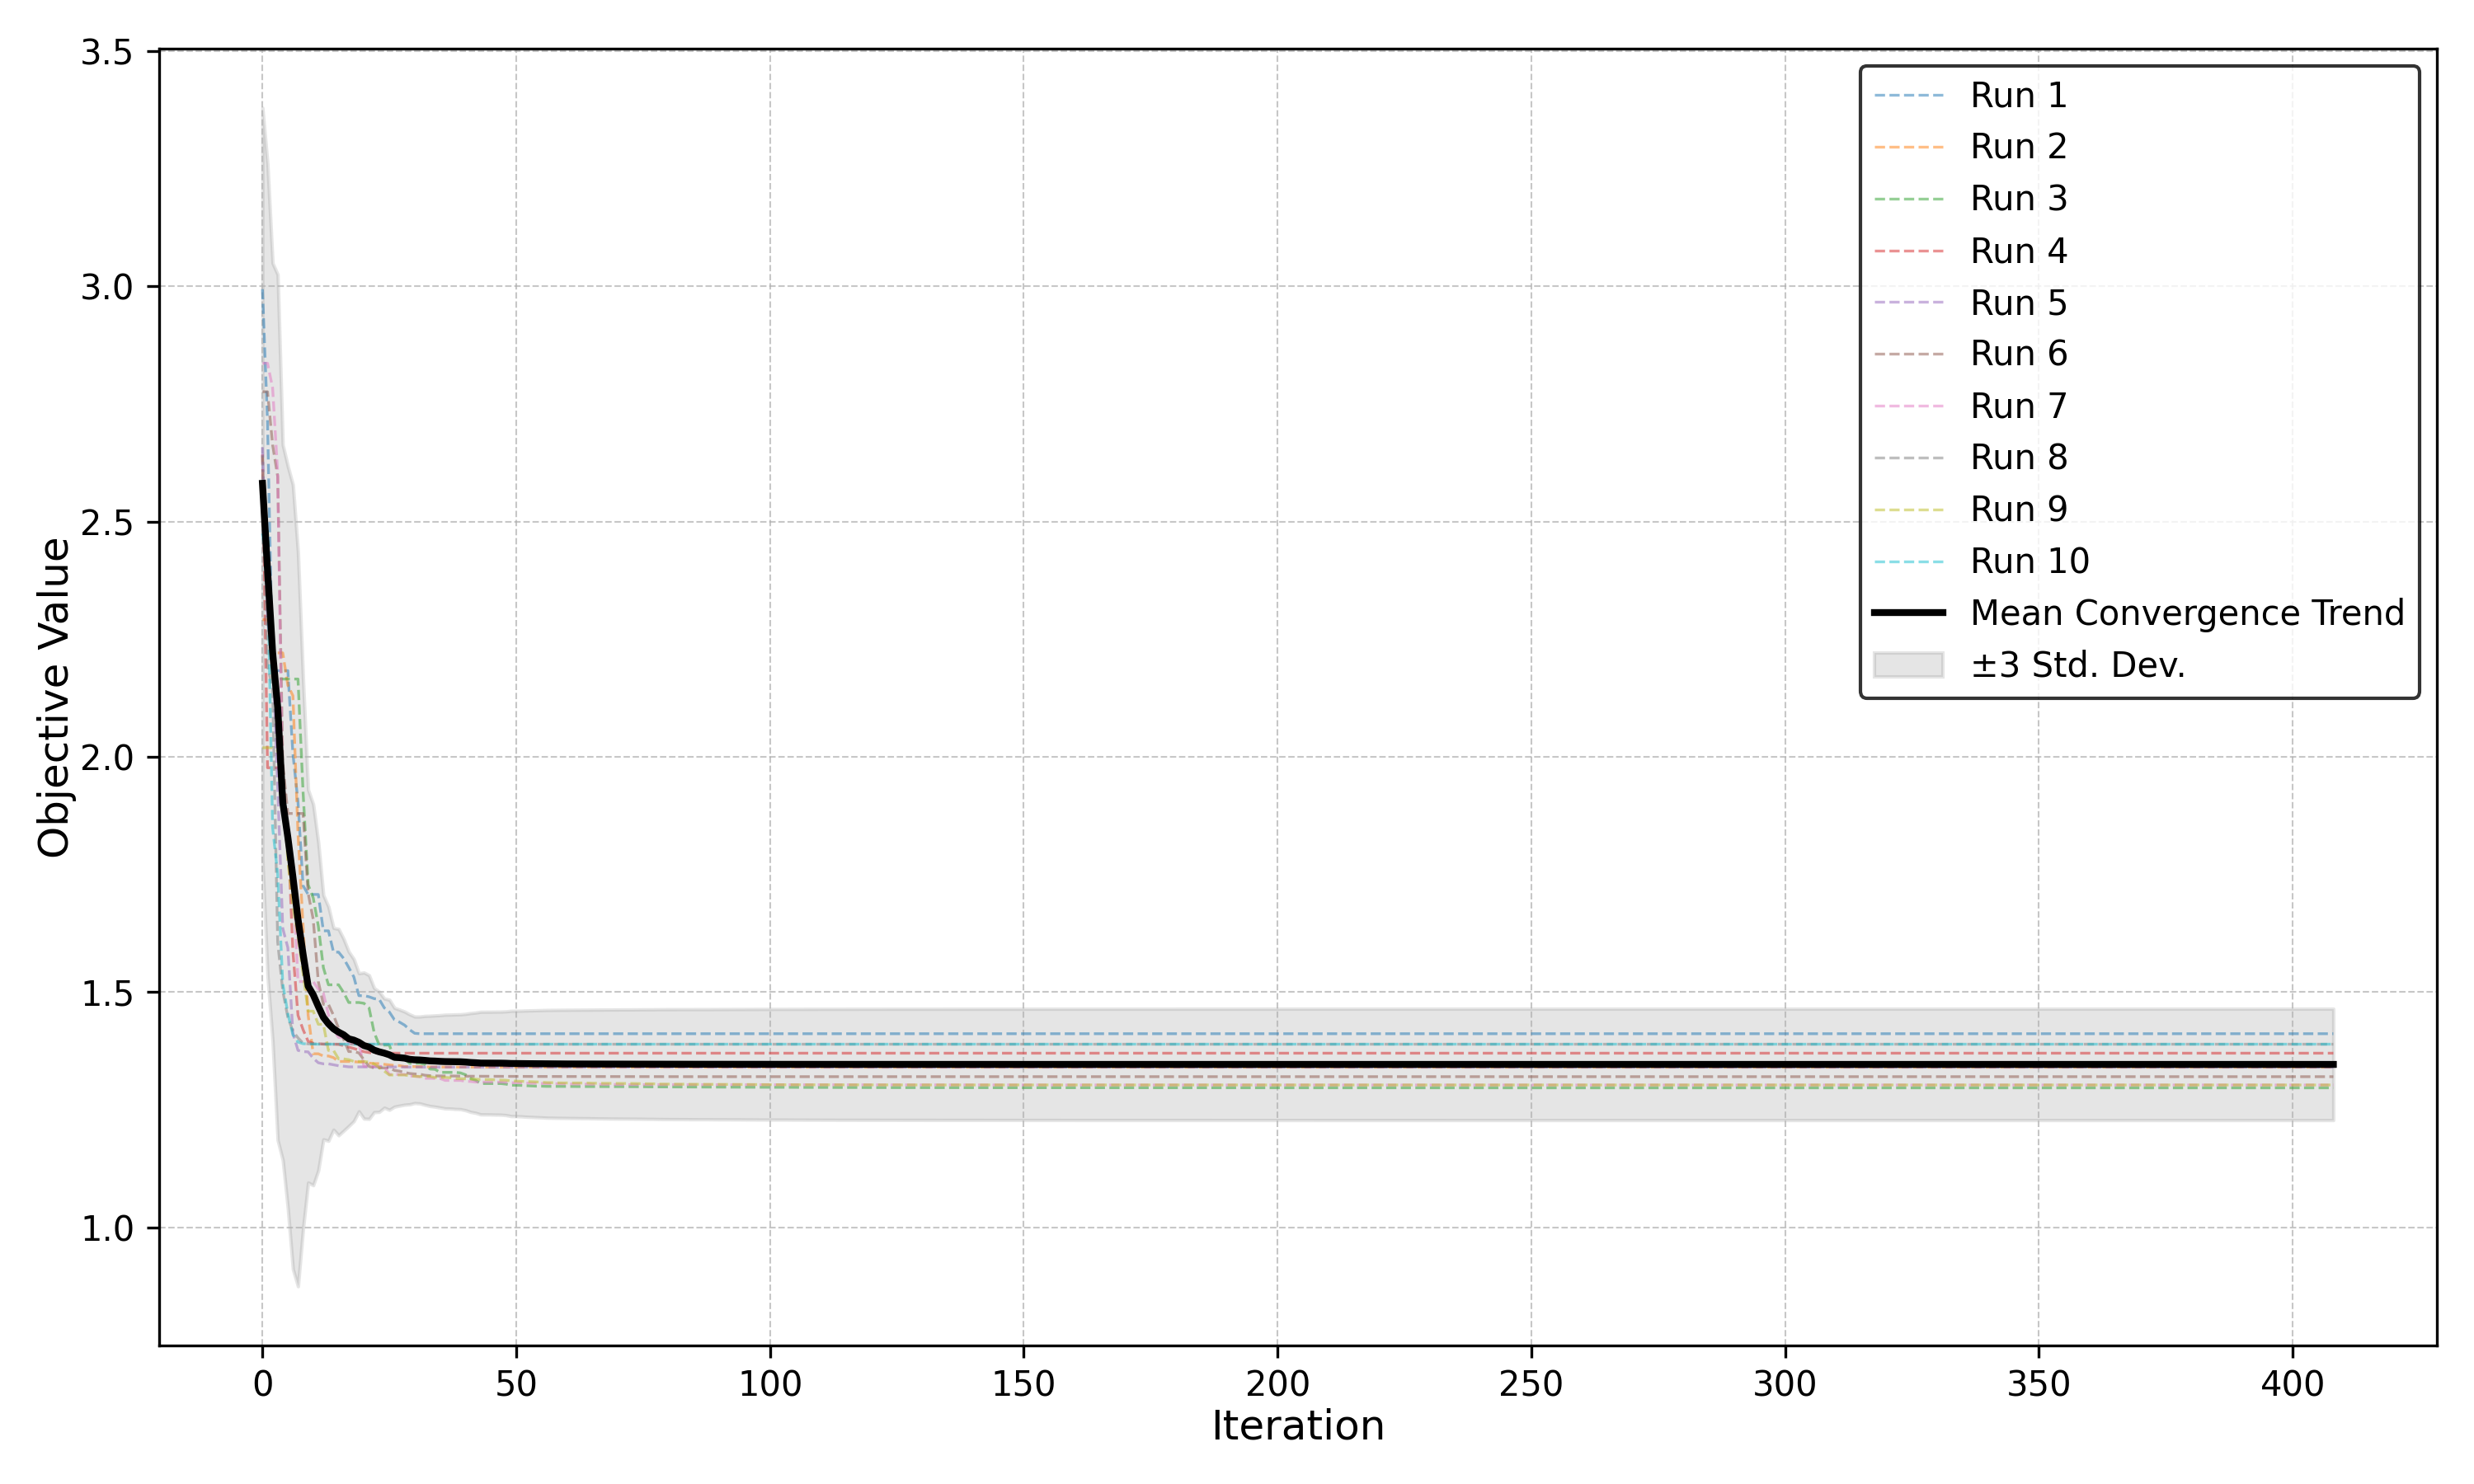
\includegraphics[width=0.7\textwidth]{../best_plots/P4_15D_convergence_n59_w0.406_c11.527_c22.135_STATIC_rho7535.png}
    \caption{Convergence plot for the brachistochrone problem with $n=15$.}
    \label{fig:P4_convergence_n15}
\end{figure}

\begin{figure}[h!]
    \centering
    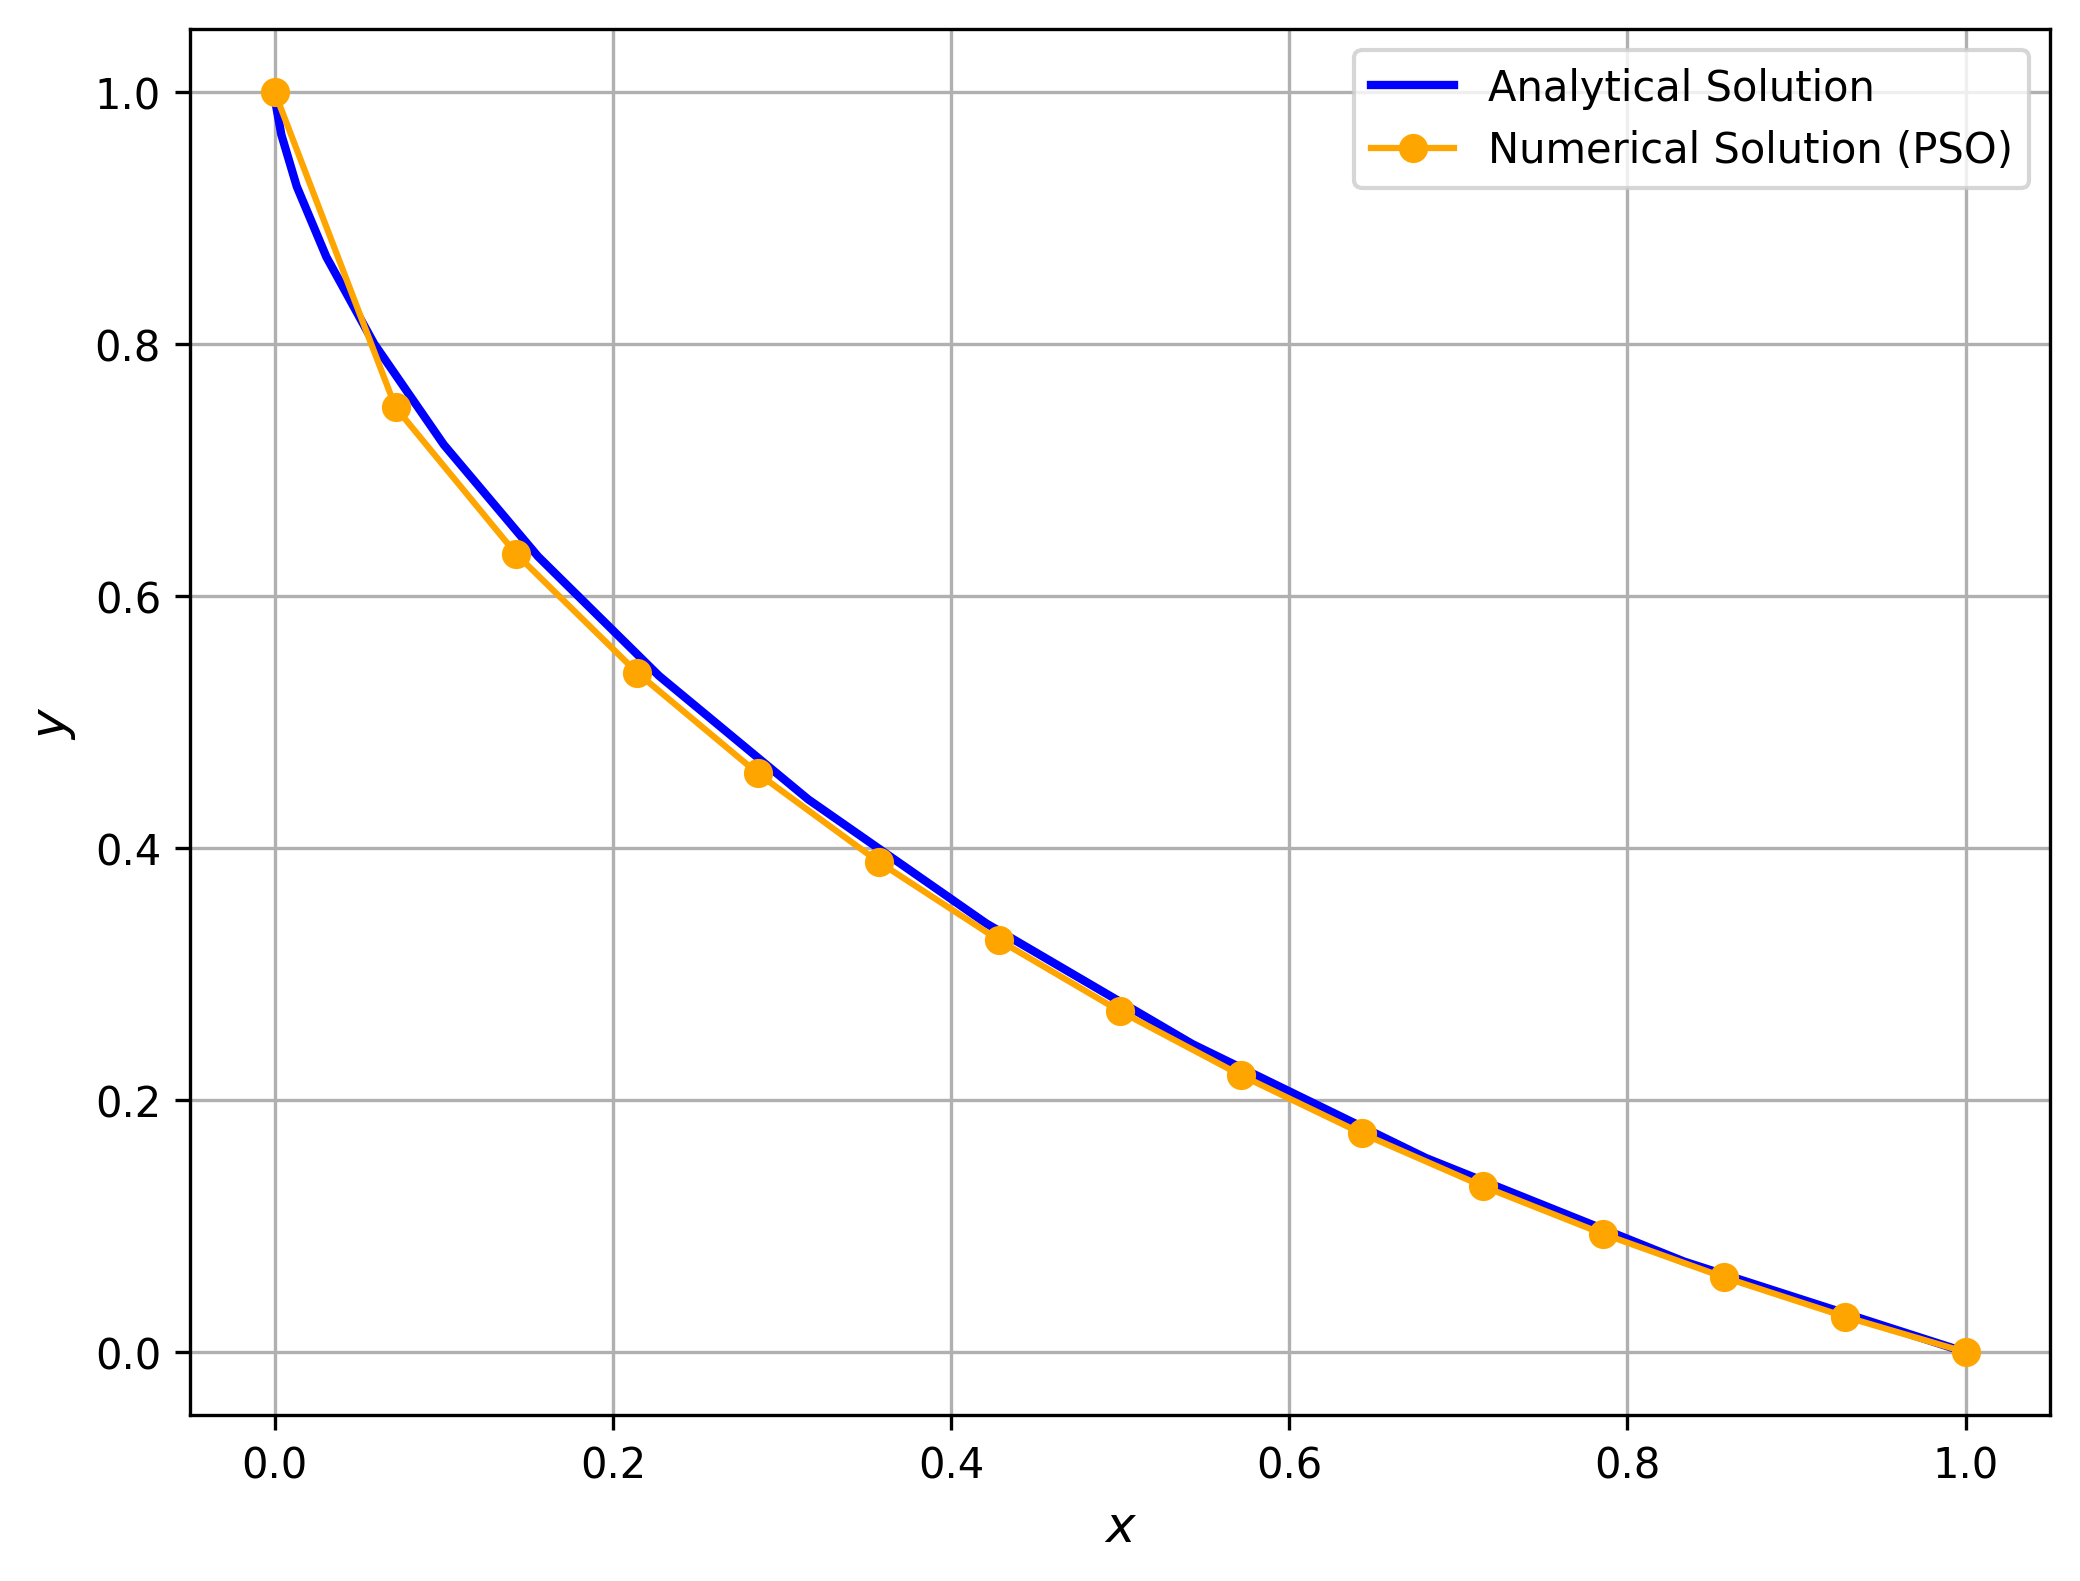
\includegraphics[width=0.5\textwidth]{../best_plots/P4_comparison_n15.png}
    \caption{Comparison of numerical and analytical solutions for the brachistochrone problem with $n=15$.}
    \label{fig:P4_comparison_n15}
\end{figure}

\paragraph{Results for $n=30$}
The best solution obtained for $n=30$ is:
\begin{align*}
    \mathbf{y} = \begin{bmatrix}
        0.8398, 0.7631, 0.6988, 0.6446, 0.5947, 0.5499, 0.5094, 0.4717, 0.4370, 0.4049,\\
        0.3752, 0.3479, 0.3211, 0.2963, 0.2728, 0.2499, 0.2272, 0.2056, 0.1845, \\
        0.1641, 0.1447, 0.1258, 0.1067, 0.0881, 0.0690, 0.0511, 0.0336, 0.0167
    \end{bmatrix}.
\end{align*}
The total travel time for the best solution with 30 points is:
\[
T = 1.2941.
\]
The convergence trend across 10 independent runs is shown in Figure~\ref{fig:P4_convergence_n30}, and the comparison between the numerical and analytical solutions is shown in Figure~\ref{fig:P4_comparison_n30}. The maximum difference in height $y_i$ between the numerical solution and the analytical solution is $0.019140$. 

\begin{figure}[h!]
    \centering
    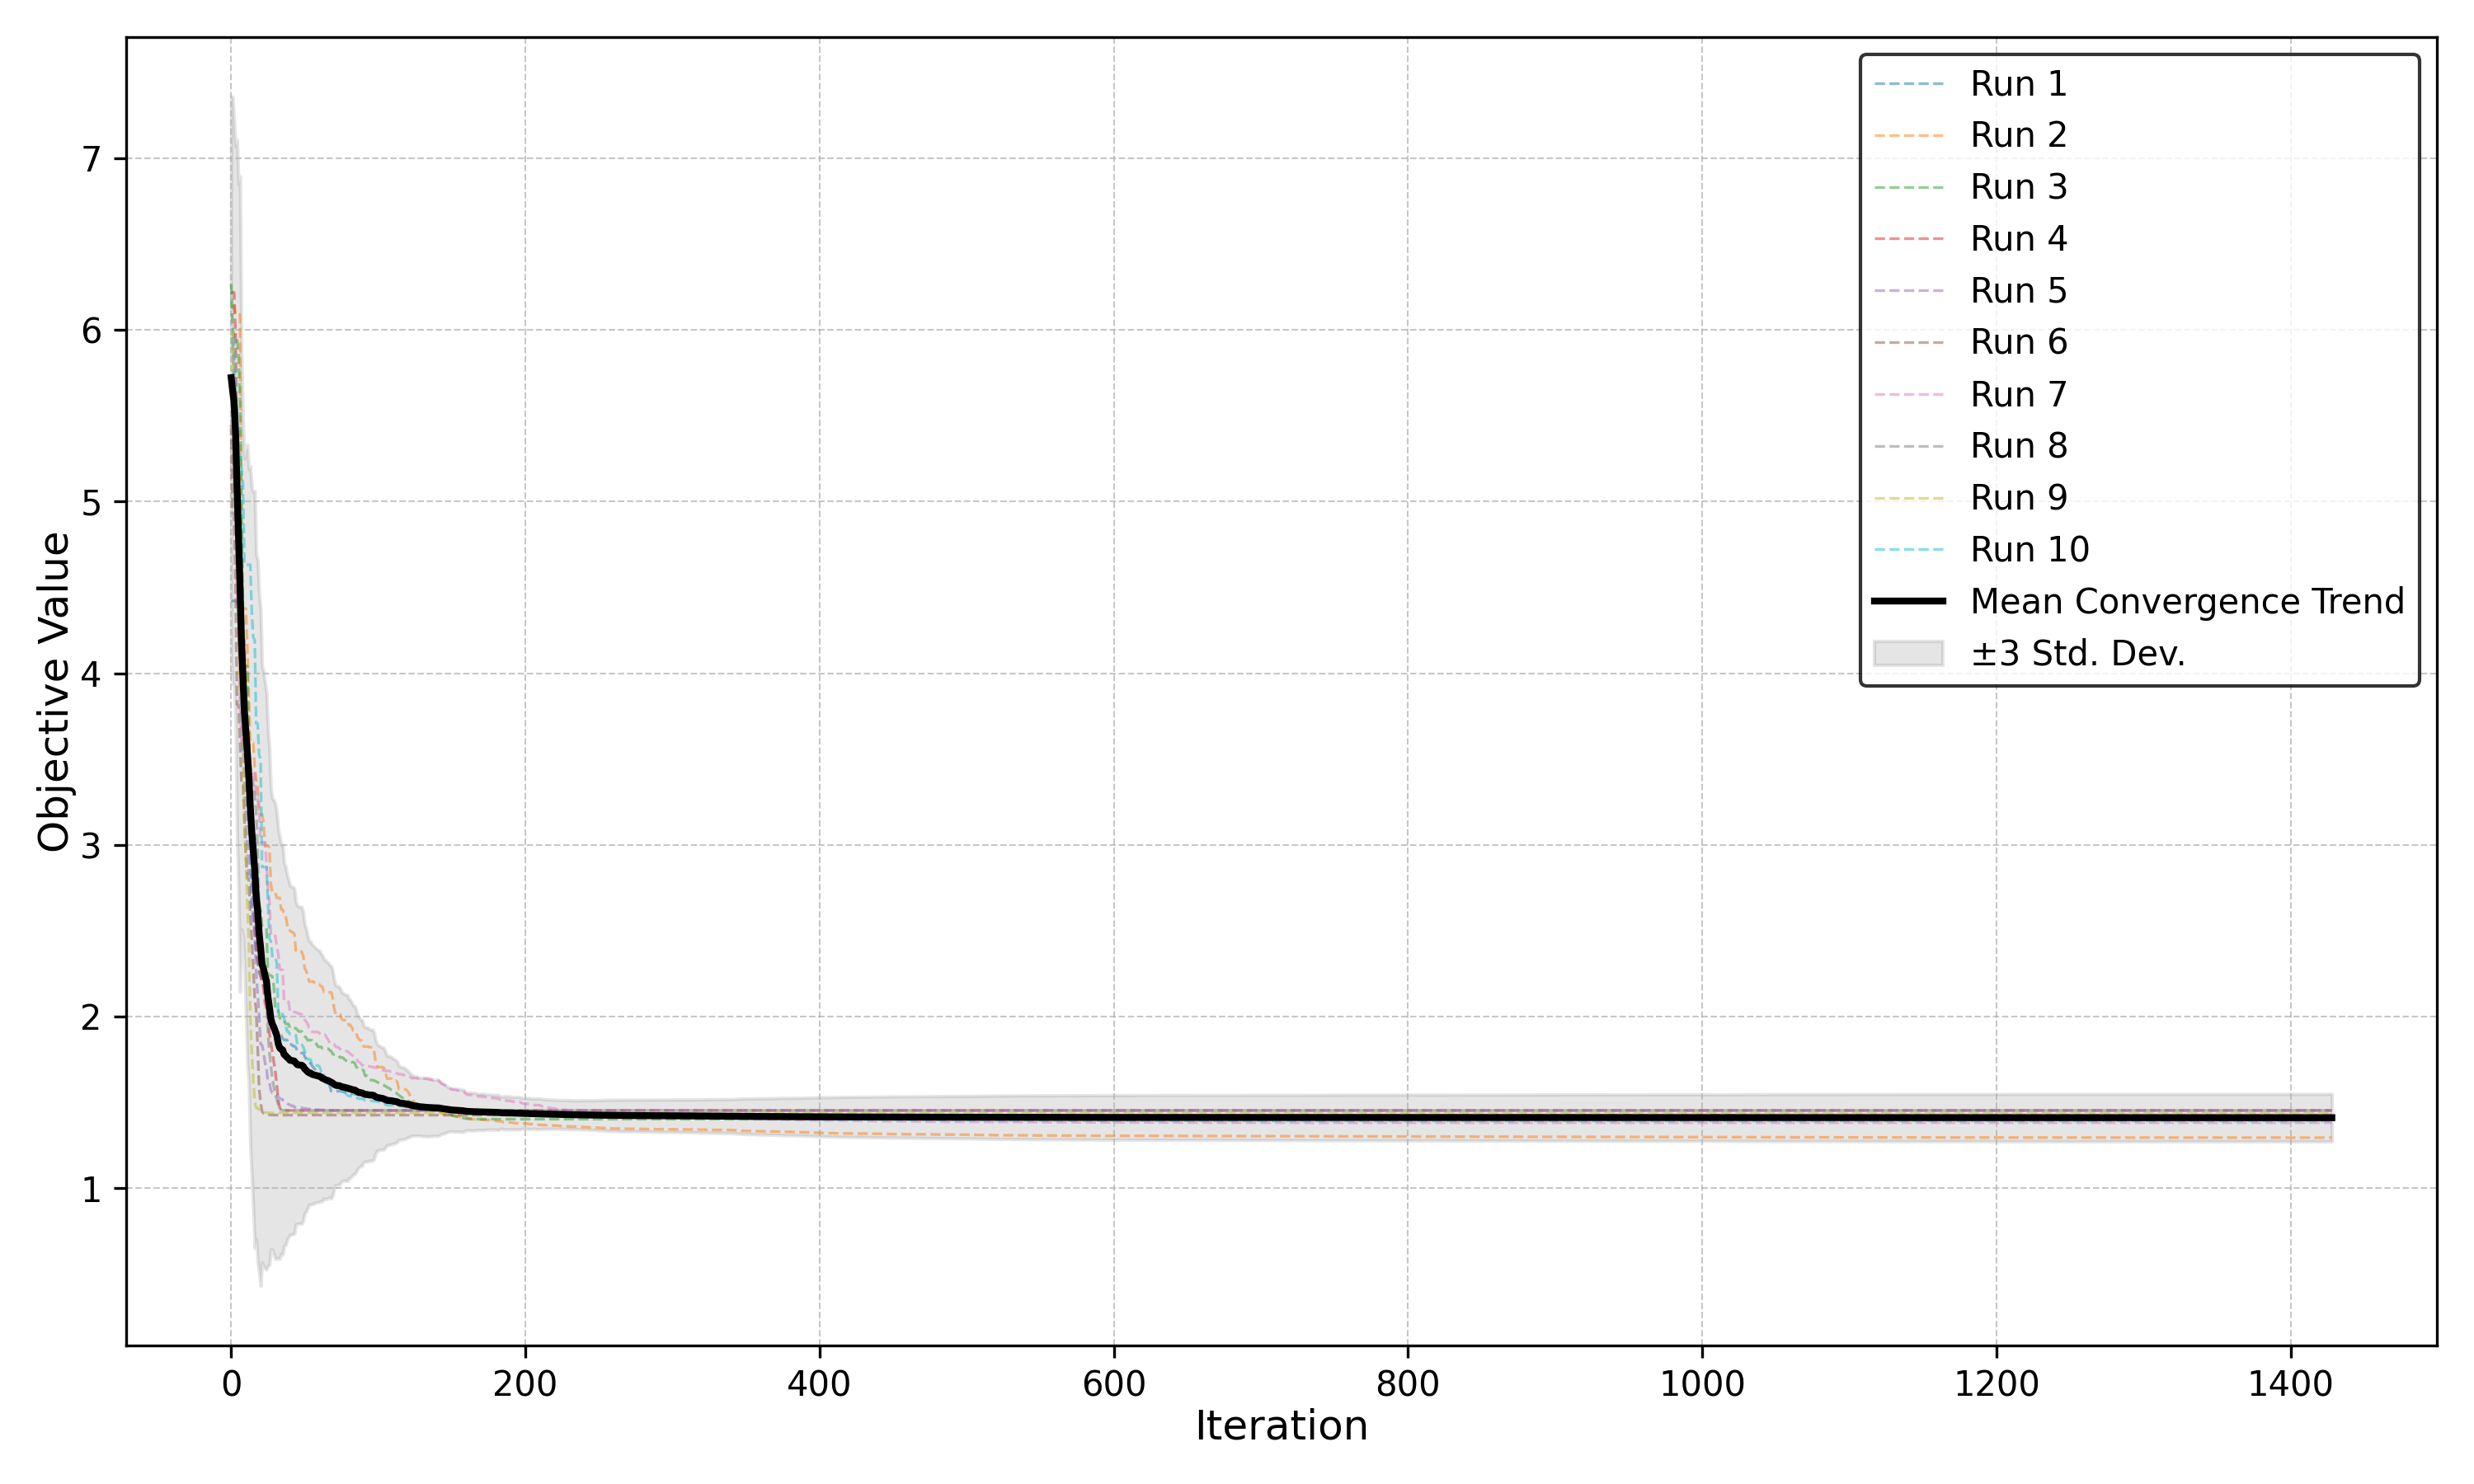
\includegraphics[width=0.7\textwidth]{../best_plots/P4_30D_convergence_n59_w0.406_c11.527_c22.135_STATIC_rho7535.png}
    \caption{Convergence plot for the brachistochrone problem with $n=30$.}
    \label{fig:P4_convergence_n30}
\end{figure}

\begin{figure}[h!]
    \centering
    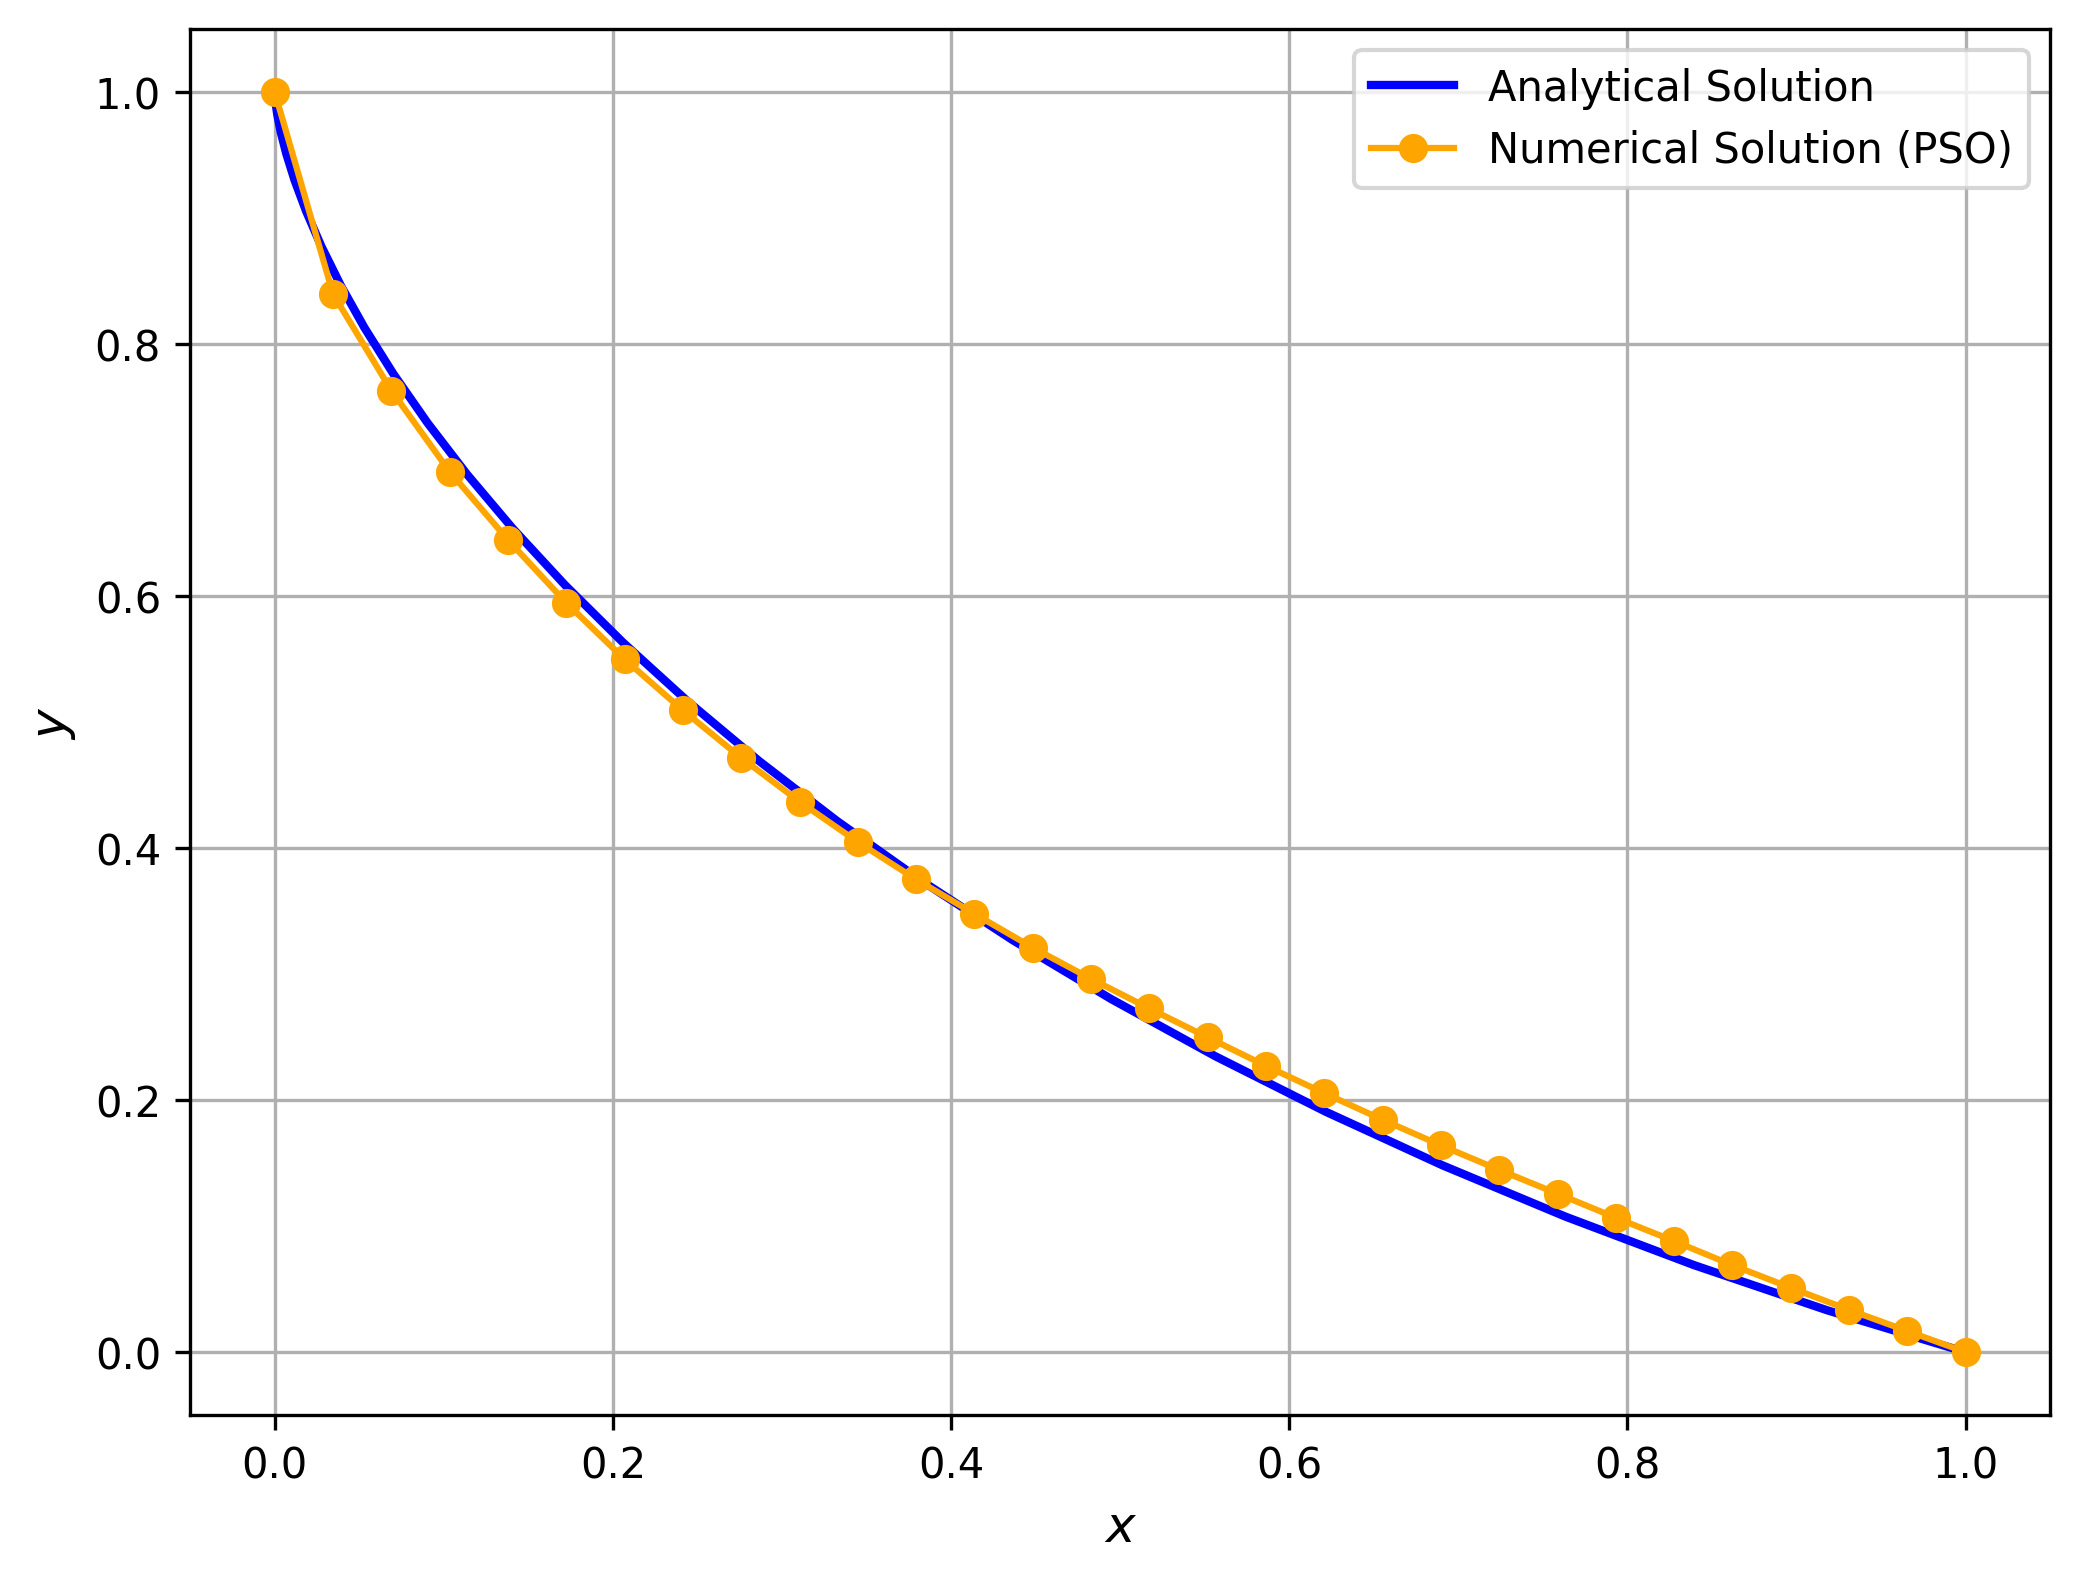
\includegraphics[width=0.5\textwidth]{../best_plots/P4_comparison_n30.png}
    \caption{Comparison of numerical and analytical solutions for the brachistochrone problem with $n=30$.}
    \label{fig:P4_comparison_n30}
\end{figure}

\paragraph{Summary}
The PSO algorithm successfully solved the brachistochrone problem for both levels of discretization. The numerical solutions closely matched the analytical solutions, with small differences observed due to the discretization and optimization process. The results validate the effectiveness of PSO for this problem.

\subsection{P5: Estimation of Damping Factor and Stiffness}
\subsubsection{Problem Formulation}
The objective of this study is to calibrate the parameters of a viscously damped linear oscillator to match the measured response $u_\text{meas}$of the system under periodic forcing. The analytical response of the oscillator is given by:
\begin{align*}
    u(t) = \left(A \cos(\omega_d t) + B \sin(\omega_d t)\right) e^{-\frac{c}{2m}t} + \frac{F_0}{C} \cos(\omega t - \alpha),
\end{align*}
where:
\begin{itemize}
    \item $m = 1$ is the mass,
    \item $k$ is the stiffness (unknown),
    \item $c$ is the damping coefficient (unknown),
    \item $\omega=0.1$ is the forcing frequency,
    \item $F_0=1$ is the forcing amplitude,
    \item $\omega_d = \sqrt{\frac{k}{m} - \left(\frac{c}{2m}\right)^2}$ is the damped natural frequency,
    \item $C = \sqrt{(k - m\omega^2)^2 + (c\omega)^2}$, and
    \item $\alpha = \tan^{-1}\left(\frac{c\omega}{k - m\omega^2}\right)$ is the phase angle.
\end{itemize}

The optimization problem is formulated as follows:
\begin{align*}
    \text{Find:} & \quad \arg \min_{\mathbf{x} \in \mathbb{R}^{2}}  \sum_{i=1}^N \left(u_{\text{sim}}(t_i; \mathbf{x}) - u_{\text{meas}}(t_i)\right)^2, \\
    \text{Subject to:} & \quad k \in [0.1, 100], \quad c \in [0.01, 10], \quad \frac{k}{m} - \left(\frac{c}{2m}\right)^2 \geq 0.
\end{align*}
where:
\begin{itemize}
    \item $u_{\text{sim}}(t_i; \mathbf{x})$ is the simulated displacement using parameters $\mathbf{x} = [k, c]$,
    \item $u_{\text{meas}}(t_i)$ is the measured displacement at time $t_i$, and
    \item $N=500$ is the number of time points.
\end{itemize}

\paragraph{Instability Constraint:} 
The constraint \( \frac{k}{m} - \left(\frac{c}{2m}\right)^2 \geq 0 \) ensures that the damped natural frequency \( \omega_d \) is well-defined (i.e., the argument inside the square root remains non-negative). If this constraint is violated, the analytical solution is not physically meaningful, leading to numerical instabilities such as NaN values. The constraint is therefore enforced in the optimization process to ensure valid system parameters.


\paragraph{Choice of Bounds:} The bounds for the parameters were chosen based on their physical meaning and practical engineering ranges:
\begin{itemize}
    \item $k$ (stiffness): Set to $[0.1, 100]$, covering a wide range from soft springs to very stiff ones.
    \item $c$ (damping coefficient): Set to $[0.01, 10]$, accounting for lightly damped to heavily damped systems.
\end{itemize}
These bounds ensure the optimization process covers realistic parameter values while avoiding non-physical or unstable solutions.

\subsubsection{Optimization Results}

The tuned Particle Swarm Optimization (PSO) algorithm was applied to estimate the stiffness $k$ and damping coefficient $c$ by minimizing the squared error between the simulated response $u_{\text{sim}}(t)$ and the measured response $u_{\text{meas}}(t)$. 

The optimization successfully converged to an optimal solution satisfying the physical constraints. The best solution obtained is:
\begin{align*}
    k^* &= 10.2034, \\
    c^* &= 0.7997.
\end{align*}
The corresponding objective function value (sum of squared errors) is:
\begin{align*}
    J^* &= 0.000376.
\end{align*}

The convergence plot for the PSO optimization process is shown in Figure~\ref{fig:P5_convergence}, illustrating the reduction in objective function value over iterations. The comparison between the simulated response using the optimized parameters and the measured response is presented in Figure~\ref{fig:P5_comparison}.

\begin{figure}[h!]
    \centering
    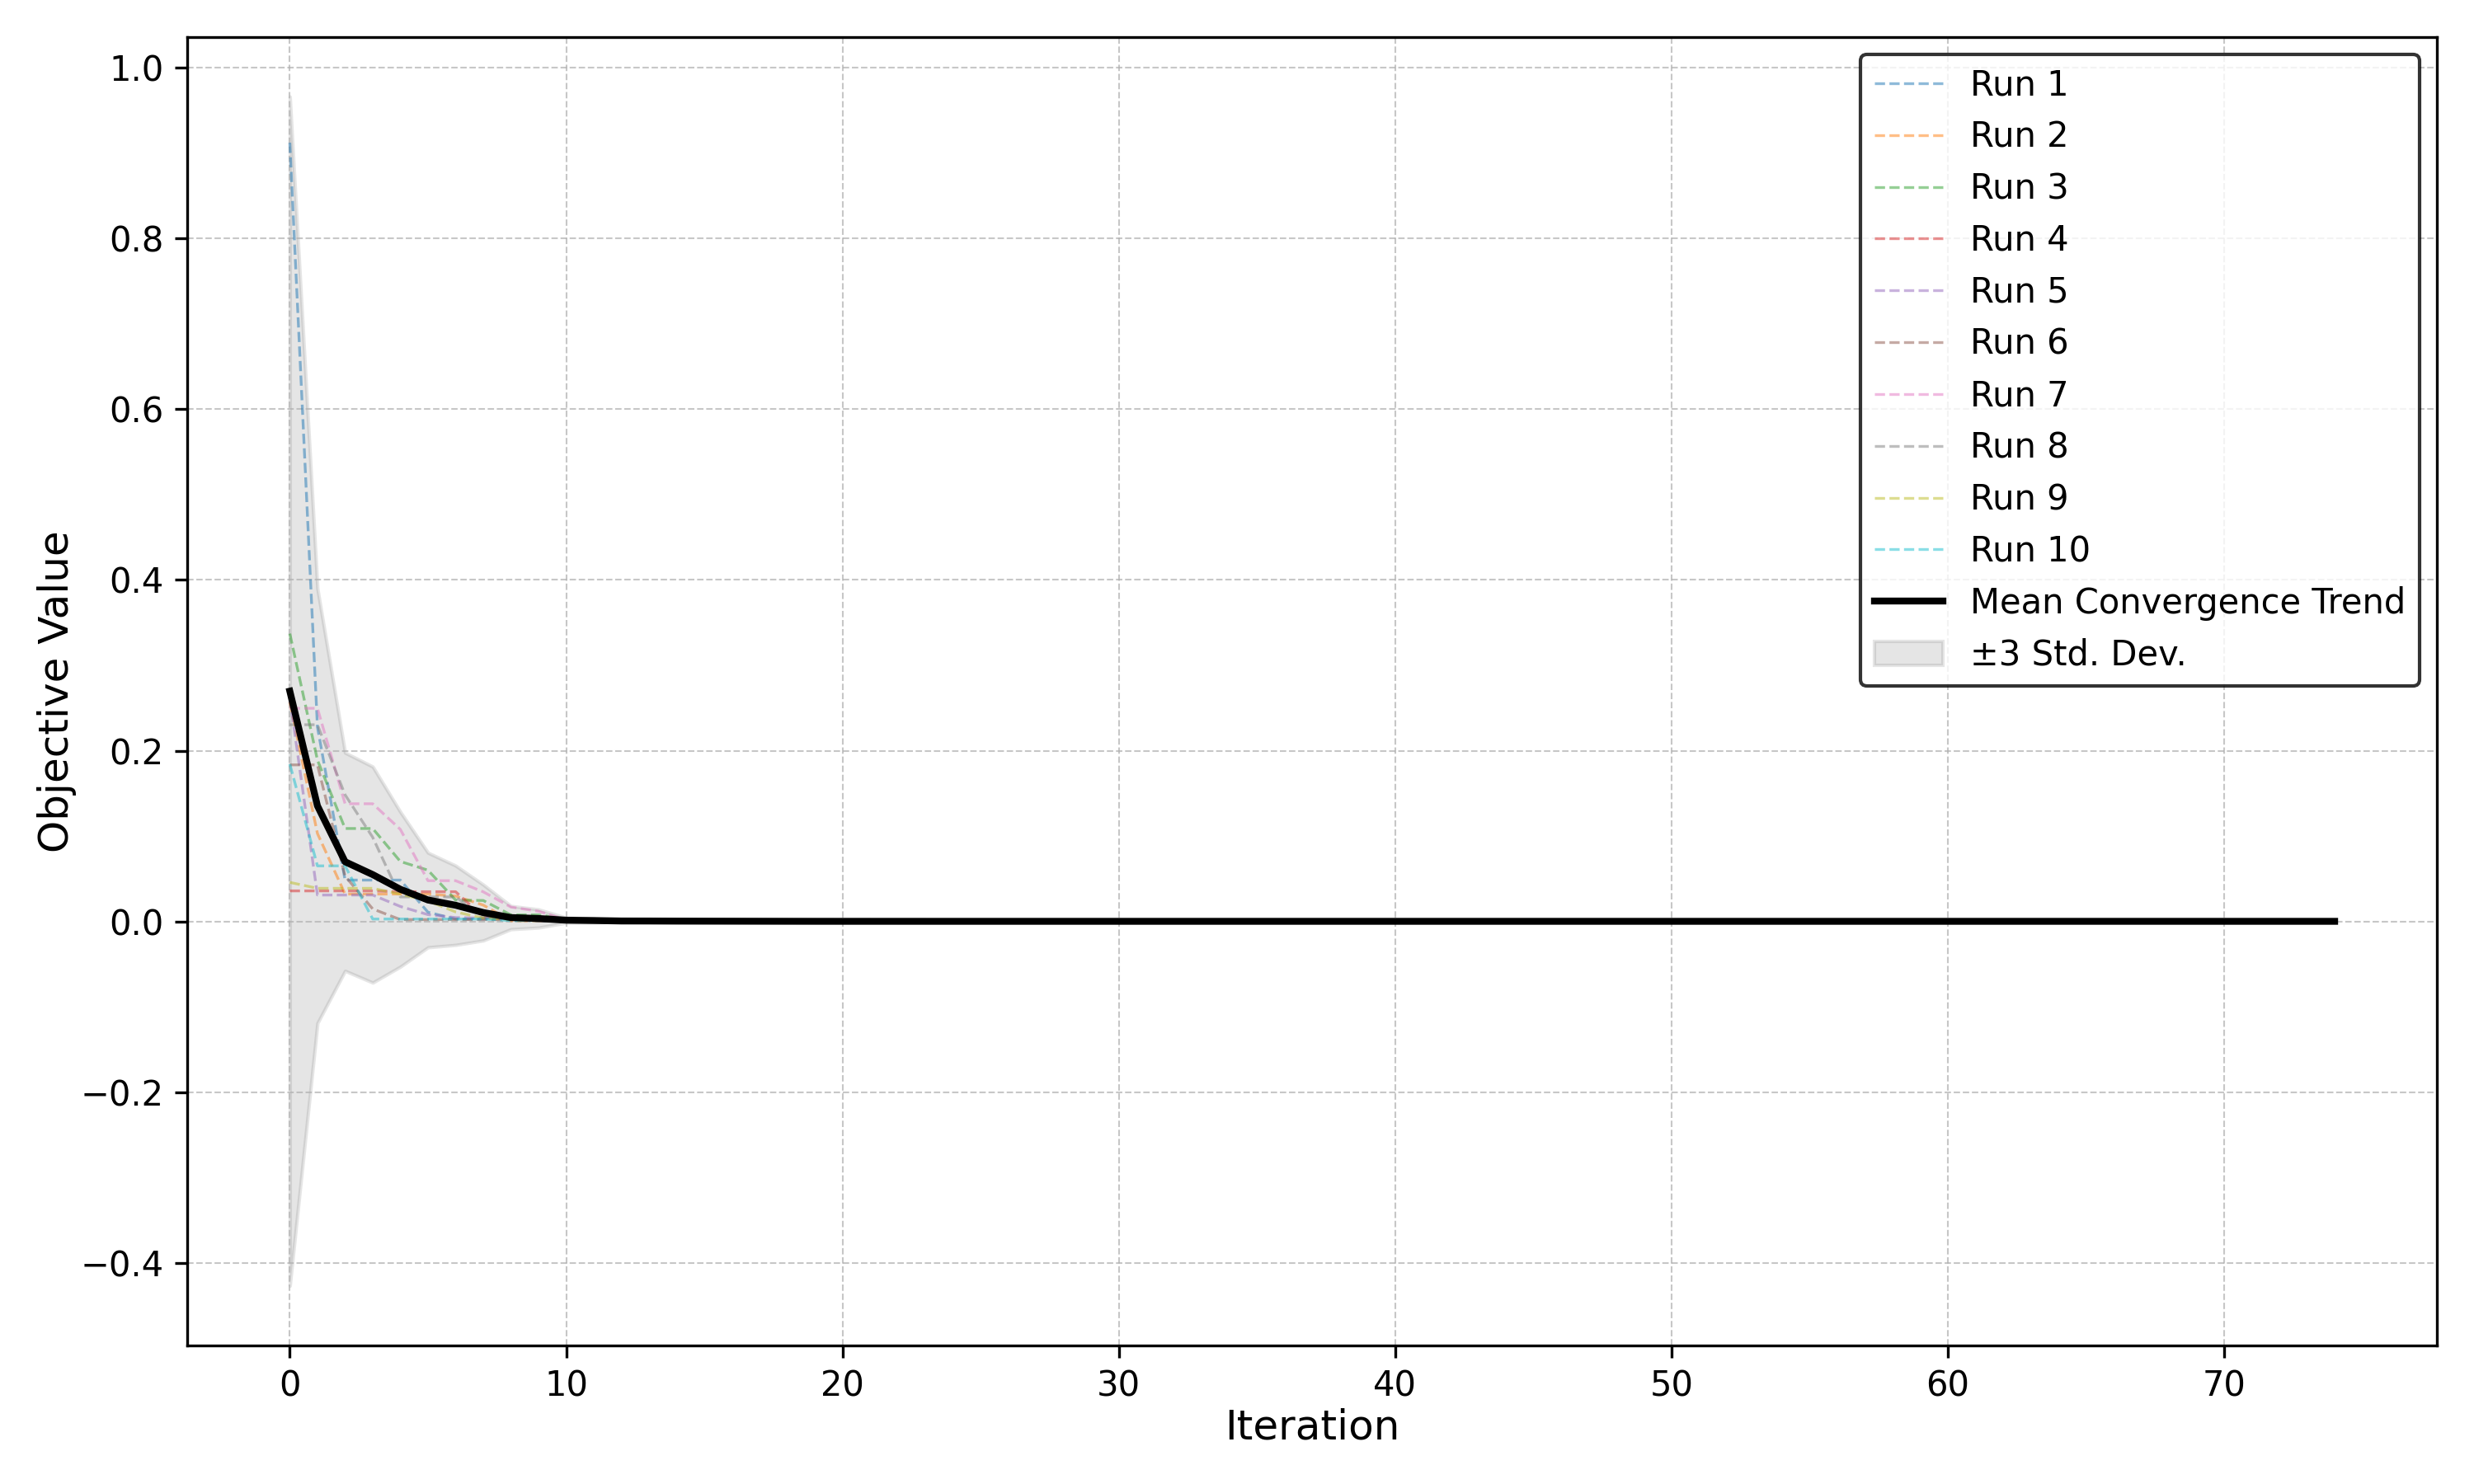
\includegraphics[width=0.7\textwidth]{../best_plots/P5_Optimization_convergence_n59_w0.406_c11.527_c22.135_STATIC_rho7535.png}
    \caption{Convergence plot for the estimation of $k$ and $c$ using PSO.}
    \label{fig:P5_convergence}
\end{figure}

\begin{figure}[h!]
    \centering
    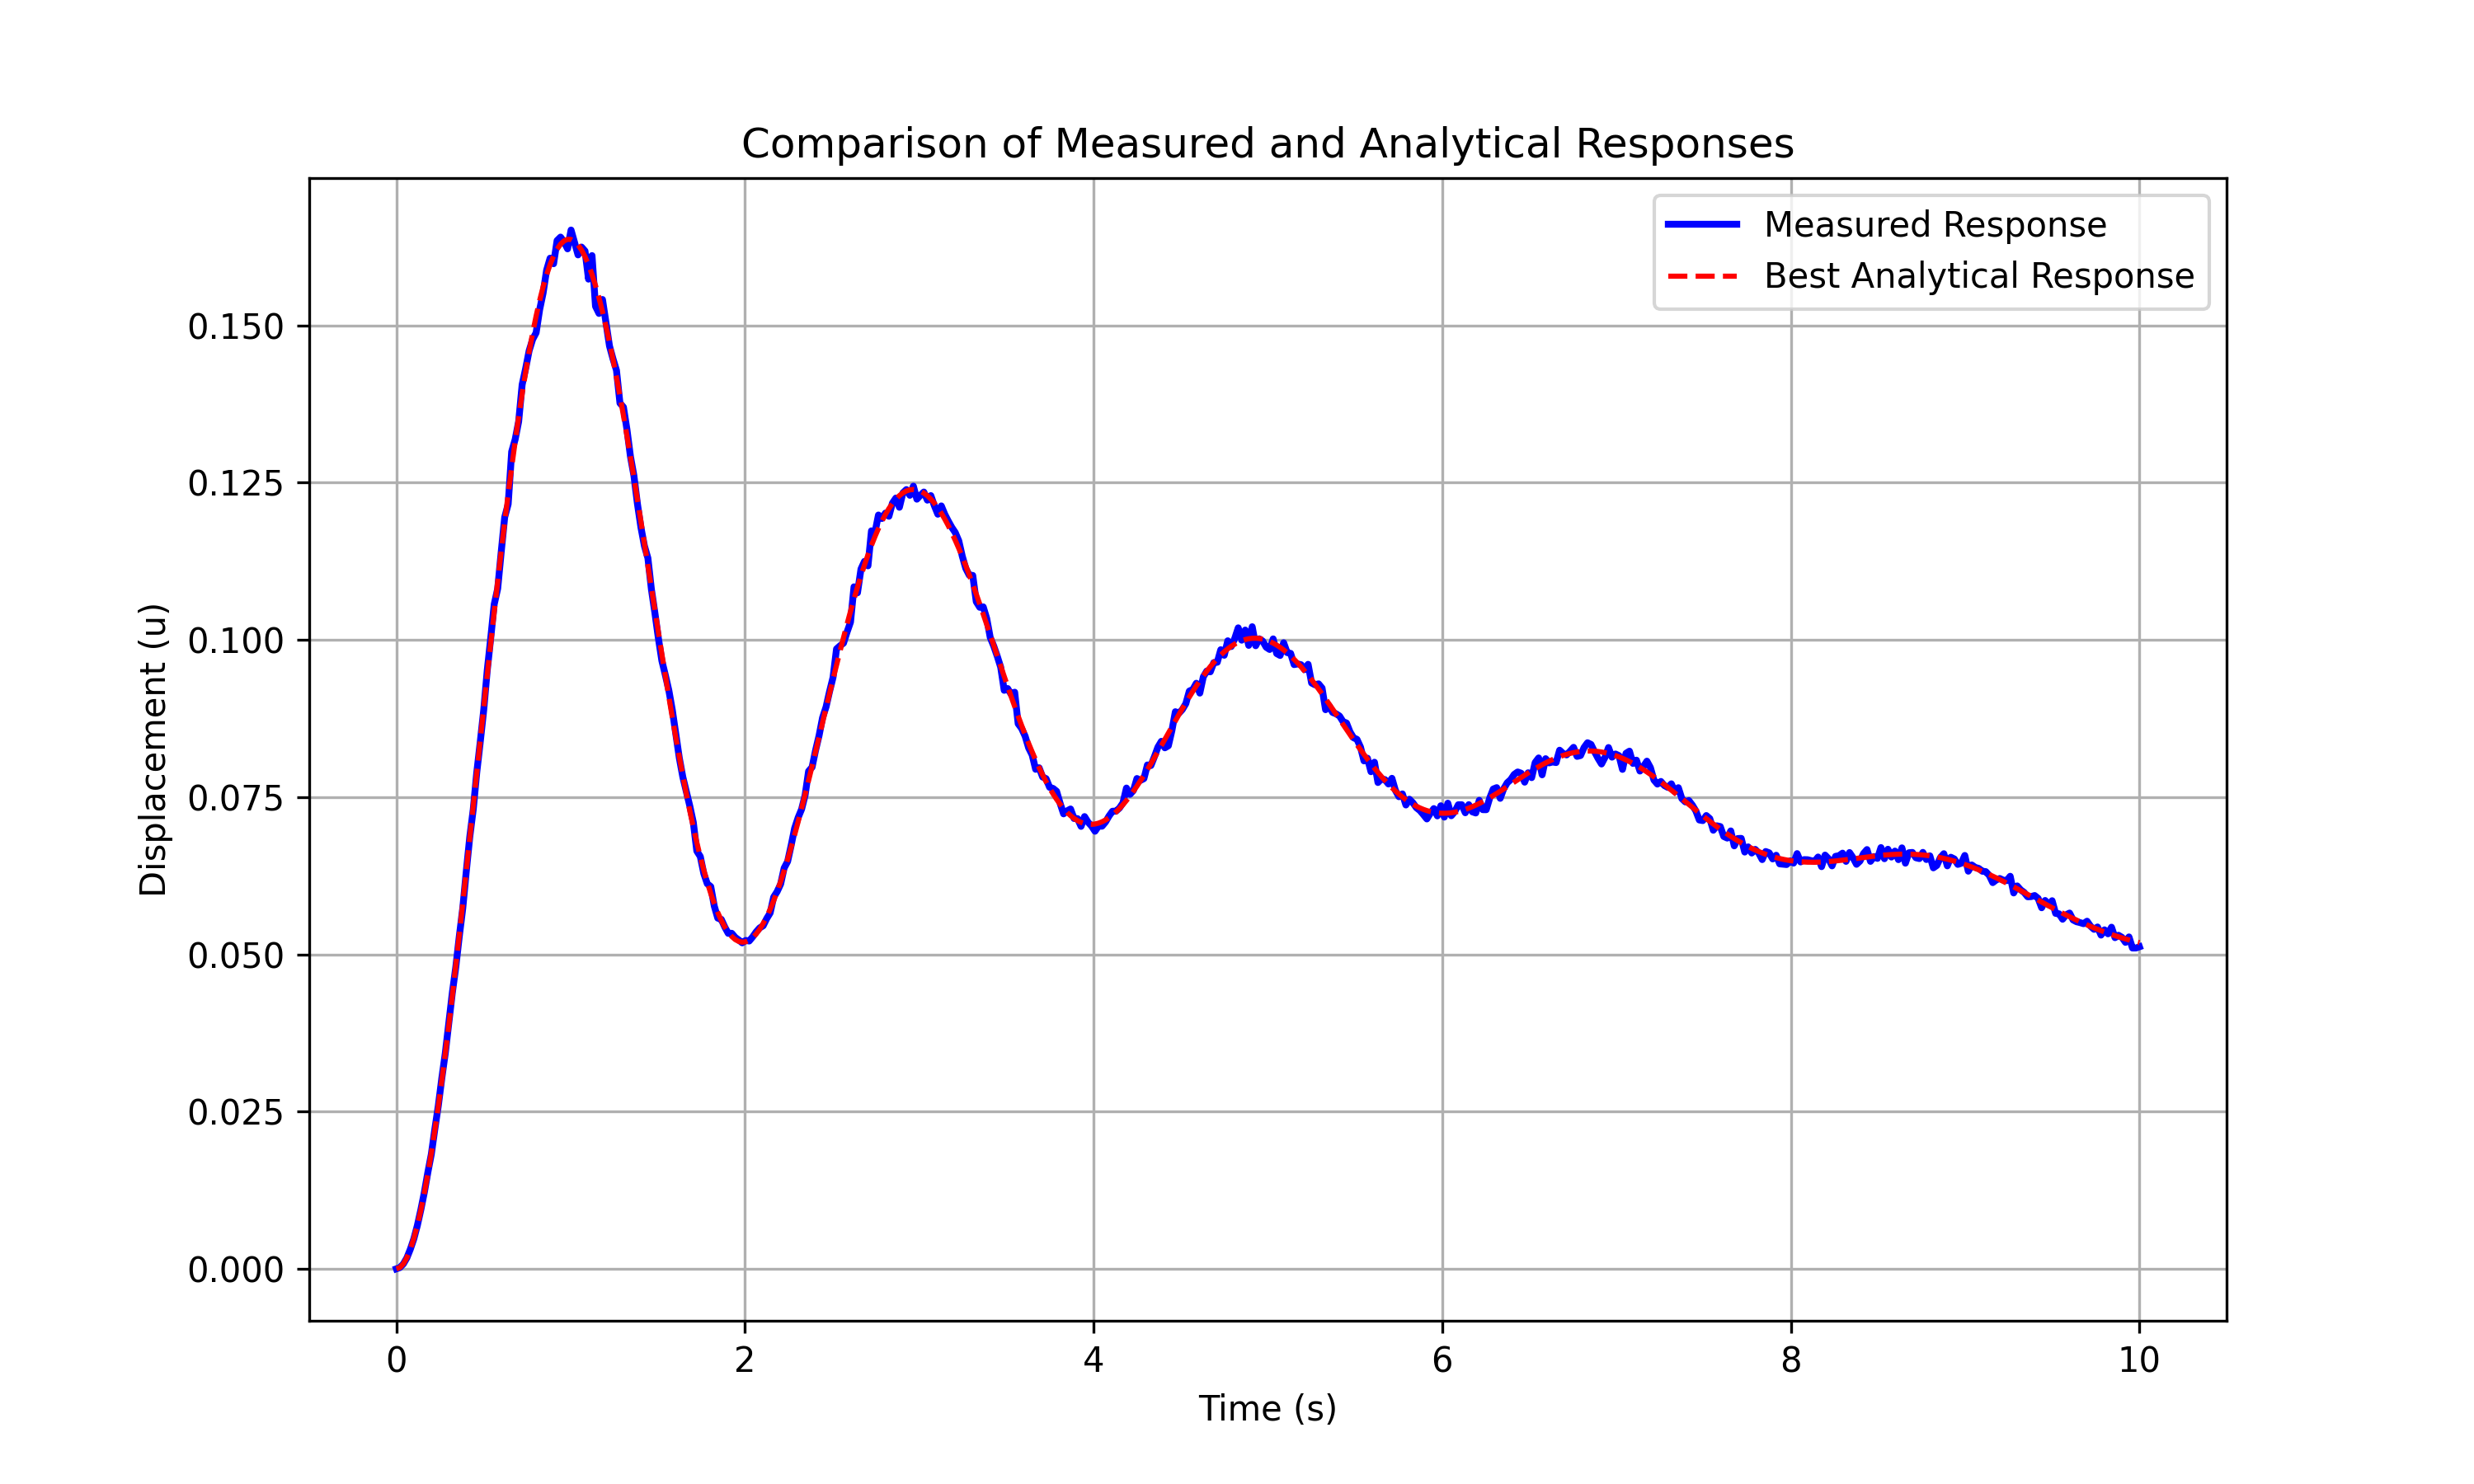
\includegraphics[width=0.9\textwidth]{../best_plots/P5_comparison.png}
    \caption{Comparison between the measured response and the simulated response using the optimized parameters.}
    \label{fig:P5_comparison}
\end{figure}

\section{Regression Problem}

We start with the given regression model:

\begin{align*}
    \hat{f}(\mathbf{x}, \mathbf{w}) &= w_0 + \sum_{i=1}^{M-1} w_i \phi_i(\mathbf{x}).
\end{align*}

Given a dataset \( \{(\mathbf{x}^{(i)}, y^{(i)})\}_{i=1}^{N} \), we seek to determine the optimal weights \( \mathbf{w} \) by minimizing the following regularized weighted least-squares objective function:

\begin{align*}
    J(\mathbf{w}) = \sum_{i=1}^{N} c_i \left( \hat{f}(\mathbf{x}^{(i)}, \mathbf{w}) - y^{(i)} \right)^2 + \sum_{i=1}^{M-1} \lambda_i w_i^2,
\end{align*}

where \( c_i > 0 \) are user-defined weights and \( \lambda_i > 0 \) are regularization parameters.

\subsection{Matrix Formulation}

We introduce the following matrix definitions:
\[
    \mathbf{\Phi} =
    \begin{bmatrix}
        1 & \phi_1(\mathbf{x}^{(1)}) & \phi_2(\mathbf{x}^{(1)}) & \dots & \phi_{M-1}(\mathbf{x}^{(1)}) \\
        1 & \phi_1(\mathbf{x}^{(2)}) & \phi_2(\mathbf{x}^{(2)}) & \dots & \phi_{M-1}(\mathbf{x}^{(2)}) \\
        \vdots & \vdots & \vdots & \ddots & \vdots \\
        1 & \phi_1(\mathbf{x}^{(N)}) & \phi_2(\mathbf{x}^{(N)}) & \dots & \phi_{M-1}(\mathbf{x}^{(N)})
    \end{bmatrix} \in \mathbb{R}^{N \times M}
\]
\begin{align*}
    \mathbf{w} &=
    \begin{bmatrix}
        w_0 & w_1 & w_2 & \cdots & w_{M-1}
    \end{bmatrix}^T \in \mathbb{R}^{M}
\\
    \mathbf{y} &=
    \begin{bmatrix}
        y^{(1)} &
        y^{(2)} &
        \cdots &
        y^{(N)}
    \end{bmatrix}^T \in \mathbb{R}^{N}
\\
    \mathbf{C} &= \text{diag}(c_1, c_2, \dots, c_N) \in \mathbb{R}^{N \times N}
\\
    \mathbf{\Lambda} &= \text{diag}(0, \lambda_1, \lambda_2, \dots, \lambda_{M-1}) \in \mathbb{R}^{M \times M}
\end{align*}

\subsection{Rewriting the Objective Function}

In matrix notation, the objective function can be rewritten as:
\begin{align*}
    J(\mathbf{w}) = \|\mathbf{C}^{1/2} (\mathbf{\Phi} \mathbf{w} - \mathbf{y})\|_2^2 + \mathbf{w}^T \mathbf{\Lambda} \mathbf{w}.
\end{align*}

Expanding the first term:
\begin{align*}
    J(\mathbf{w}) = (\mathbf{\Phi} \mathbf{w} - \mathbf{y})^T \mathbf{C} (\mathbf{\Phi} \mathbf{w} - \mathbf{y}) + \mathbf{w}^T \mathbf{\Lambda} \mathbf{w}.
\end{align*}

\subsection{Computing the Gradient}

Expanding the squared term:
\begin{align*}
    (\mathbf{\Phi} \mathbf{w} - \mathbf{y})^T \mathbf{C} (\mathbf{\Phi} \mathbf{w} - \mathbf{y}) &= \mathbf{w}^T \mathbf{\Phi}^T \mathbf{C} \mathbf{\Phi} \mathbf{w} - 2 \mathbf{y}^T \mathbf{C} \mathbf{\Phi} \mathbf{w} + \mathbf{y}^T \mathbf{C} \mathbf{y}.
\end{align*}

Taking the gradient with respect to \( \mathbf{w} \):

1. First term:
\begin{align*}
    \nabla_{\mathbf{w}} \left( \mathbf{w}^T \mathbf{\Phi}^T \mathbf{C} \mathbf{\Phi} \mathbf{w} \right) = 2 \mathbf{\Phi}^T \mathbf{C} \mathbf{\Phi} \mathbf{w}.
\end{align*}

2. Second term:
\begin{align*}
    \nabla_{\mathbf{w}} \left( -2 \mathbf{y}^T \mathbf{C} \mathbf{\Phi} \mathbf{w} \right) = -2 \mathbf{\Phi}^T \mathbf{C} \mathbf{y}.
\end{align*}

3. Third term:
\begin{align*}
    \nabla_{\mathbf{w}} (\mathbf{y}^T \mathbf{C} \mathbf{y}) = 0.
\end{align*}

4. Regularization term:
\begin{align*}
    \nabla_{\mathbf{w}} (\mathbf{w}^T \mathbf{\Lambda} \mathbf{w}) = 2 \mathbf{\Lambda} \mathbf{w}.
\end{align*}

Summing all terms:
\begin{align*}
    \nabla_{\mathbf{w}} J(\mathbf{w}) = 2 \mathbf{\Phi}^T \mathbf{C} \mathbf{\Phi} \mathbf{w} - 2 \mathbf{\Phi}^T \mathbf{C} \mathbf{y} + 2 \mathbf{\Lambda} \mathbf{w}.
\end{align*}
Setting the gradient to zero for minimization:
\begin{align*}
    2 \mathbf{\Phi}^T \mathbf{C} \mathbf{\Phi} \mathbf{w} - 2 \mathbf{\Phi}^T \mathbf{C} \mathbf{y} + 2 \mathbf{\Lambda} \mathbf{w} = 0.
\end{align*}

By rearranging the terms and simplifying, we get the desired system of equations:
\begin{align*}
    (\mathbf{\Phi}^T \mathbf{C} \mathbf{\Phi} + \mathbf{\Lambda}) \mathbf{w} = \mathbf{\Phi}^T \mathbf{C} \mathbf{y}.
\end{align*}

\subsection{Solution for \( \mathbf{w} \)}

To solve for the optimal weights \( \mathbf{w^*} \), we can use Cholesky or QR factorization or singular value decomposition (SVD) depending on the rank of the left hand side matrix $\mathbf{\Phi}^T \mathbf{C} \mathbf{\Phi} + \mathbf{\Lambda}$:
\begin{align*}
    \mathbf{w^*} = (\mathbf{\Phi}^T \mathbf{C} \mathbf{\Phi} + \mathbf{\Lambda})^{-1} \mathbf{\Phi}^T \mathbf{C} \mathbf{y}.
\end{align*}

\section{Constraint Relaxation Optimization Problem}
Consider the constrained optimization problem:
\begin{align*}
    &\min_{\mathbf{x} \in \mathbb{R}^n} f(\mathbf{x}) \\
    \text{subject to: } & g_j(\mathbf{x}) \leq 0, \quad j = 1,2,\dots,m.
\end{align*}

It is given that the feasible set is empty. We introduce the vector $\boldsymbol{\delta} = (\delta_1, \delta_2, \dots, \delta_m)^T \in \mathbb{R}^m$ with relaxation parameters $\delta_j \geq 0$ to modify the constraints as follows:
\begin{align*}
    g_j(\mathbf{x}) \leq \delta_j, \quad j = 1,2,\dots,m.
\end{align*}
The notation $\boldsymbol{\delta} \geq 0$ means that each component satisfies $\delta_j \geq 0$ for all $j$.

\subsection{Minimizing the Total Relaxation}
To find the smallest possible values of $\delta_j$ such that the feasible set is non-empty, we formulate the optimization problem:
\begin{align*}
    &\min_{\boldsymbol{\delta} \geq 0} \sum_{j=1}^{m} \delta_j
\end{align*}
subject to the existence of $\mathbf{x} \in \mathbb{R}^n$ satisfying:
\begin{align*}
    g_j(\mathbf{x}) \leq \delta_j, \quad j = 1,2,\dots,m.
\end{align*}

The objective function minimizes the sum of the relaxation parameters, which corresponds to the $\ell_1$-norm $\|\boldsymbol{\delta}\|_1 = \sum_{j=1}^{m} \delta_j$. The $\ell_1$-norm is used because it promotes sparsity in the relaxation parameters, meaning that only the most necessary constraints are relaxed. Additionally, it ensures a convex and computationally tractable optimization problem.

\subsection{Minimizing the Number of Relaxed Constraints}
To ensure feasibility while relaxing the minimum number of constraints, we introduce binary variables $z_j \in \{0,1\}$, where $z_j = 1$ if constraint $j$ is relaxed (i.e., $\delta_j > 0$). The problem is formulated as:
\begin{align*}
    &\min_{z_j \in \{0,1\}, \delta_j \geq 0} \sum_{j=1}^{m} z_j \\
    \text{subject to: } & g_j(\mathbf{x}) \leq \delta_j z_j, \quad j = 1,2,\dots,m.
\end{align*}

This formulation, however, does not differentiate between constraints that require significant relaxation and those requiring minimal adjustments. To address this, we refine the formulation by incorporating a penalty for larger relaxation values:
\begin{align*}
    &\min_{z_j \in \{0,1\}, \delta_j \geq 0} \sum_{j=1}^{m} \left( z_j + \lambda \frac{\delta_j}{\delta_{\max}} \right) \\
    \text{subject to: } & g_j(\mathbf{x}) \leq \delta_j z_j, \quad j = 1,2,\dots,m.
\end{align*}
where $\lambda > 0$ is a weighting parameter balancing the number of relaxed constraints and the magnitude of relaxation, and $\delta_{\max} = \max_j \delta_j$ ensures proper scaling.

This refined formulation ensures that constraints requiring only minor adjustments contribute less to the objective, thereby achieving a more balanced and practical relaxation strategy.

Solving these formulations poses computational challenges. The first formulation is a mixed-integer optimization problem, which is inherently combinatorial and difficult to solve efficiently for large-scale problems. The second formulation, though more balanced, introduces additional complexity due to the continuous relaxation penalty, requiring careful parameter tuning and scaling strategies to ensure numerical stability and tractability.

\subsection{Minimizing the Cost of Relaxation}
Given relaxation costs $c_j > 0$, the goal is to minimize the total cost of relaxation:
\begin{align*}
    &\min_{\boldsymbol{\delta} \geq 0} \sum_{j=1}^{m} c_j \delta_j 
\end{align*}
subject to the existence of $\mathbf{x} \in \mathbb{R}^n$ satisfying:
\begin{align*}
    g_j(\mathbf{x}) \leq \delta_j, \quad j = 1,2,\dots,m.
\end{align*}

\section{Bonus: Particle Swarm Optimization on P3 ($n=50$)}

In this bonus section, we apply the Particle Swarm Optimization (PSO) algorithm to the constrained bump test function \( P3 \) with \( n = 50 \). The best solution found, along with the corresponding optimal vector \( x^* \), is saved in the attached ASCII file \textit{best\_solution\_P3\_n50.txt}. To verify the reported solution, one can evaluate the objective function and constraints at \( x^* \) using the provided script \textit{verify\_P3\_n50.py}.


\end{document}
